\documentclass[12pt, A4]{article}
\usepackage[utf8]{inputenc}
\usepackage{graphicx}
\usepackage{geometry}
\usepackage{hyperref}
\usepackage{datetime}
\usepackage{float}
\title{Lab 2 Report}
\author{Anton Gashi: 201914462 \\ Email: \href{anton.gashi.2019@uni.strath.ac.uk}{anton.gashi.2019@uni.strath.ac.uk} \\ Github: \href{https://github.com/AntonGashi/Computation_Class}{github.com/AntonGashi/Computation\_Class}}
\date{\today}

\begin{document}
\begin{titlepage}
\clearpage\maketitle
\thispagestyle{empty}
\end{titlepage}

\section{Tasks 1 \& 2} % (fold)
\label{sec:Tasks 12}

\begin{enumerate}
  \item Write a routine which takes inputs of 1) a reference to a function to
be integrated (i.e. the integrand), 2) the limits of the integral and 3)
the number of points to sample. It should return an estimate of the
value of the integral the error in the estimate, using simple Monte
Carlo integration from the notes about definite integrals.
Think about how your function can to be written so that both
one-dimensional and multi-dimensional integrals can be evaluated.

\item Using your function, evaluate the following definite integrals, and
report the uncertainty in their evaluation. Investigate their
convergence with the number of random points (hint: you may need
to use many random numbers to get accurate values).

$$\textrm{a)}\int^1_02dx \;\; \textrm{b)}\int^1_0-xdx \;\; \textrm{c)}\int^2_{-2}x^2dx \;\; \textrm{d)}\int^1_0\int^1_0xy+xdxdy$$
\end{enumerate}

\subsection{Part a} % (fold)
\label{sub:Part a}

For part a, the answer is trivial and will always be 2 for any limit since 
the function is constant everywhere. The convergence on the answer for increasing
N is also not applicable here.

% subsection subsection name (end)

\subsection{Part b} % (fold)
\label{sub:Part b}


Integral output (to a 90\% confidence) = [-0.4999] $\pm$ 8.22e-07 units.
\\
Sample Size = [1e+06].
\\
Time Taken = [0.435]s.
\\
Variance = [0.25].
\\
Root-Mean-Square = [0.577].
\\
Standard Deviation (Of Distribution/X-axis) = [0.0005]/[0.5].

\vspace{1em}

For part b of task 2, the function $f(x)=-x$ between 0 and 1 is easily 
integrated for any reasonable amount of points. Even the first point 
on figure \ref{fig:task_2_b} using a thousand random points is only 
$\approx 3.4\%$ off the right answer of -0.5.

\begin{figure}[H]
  \begin{center}
    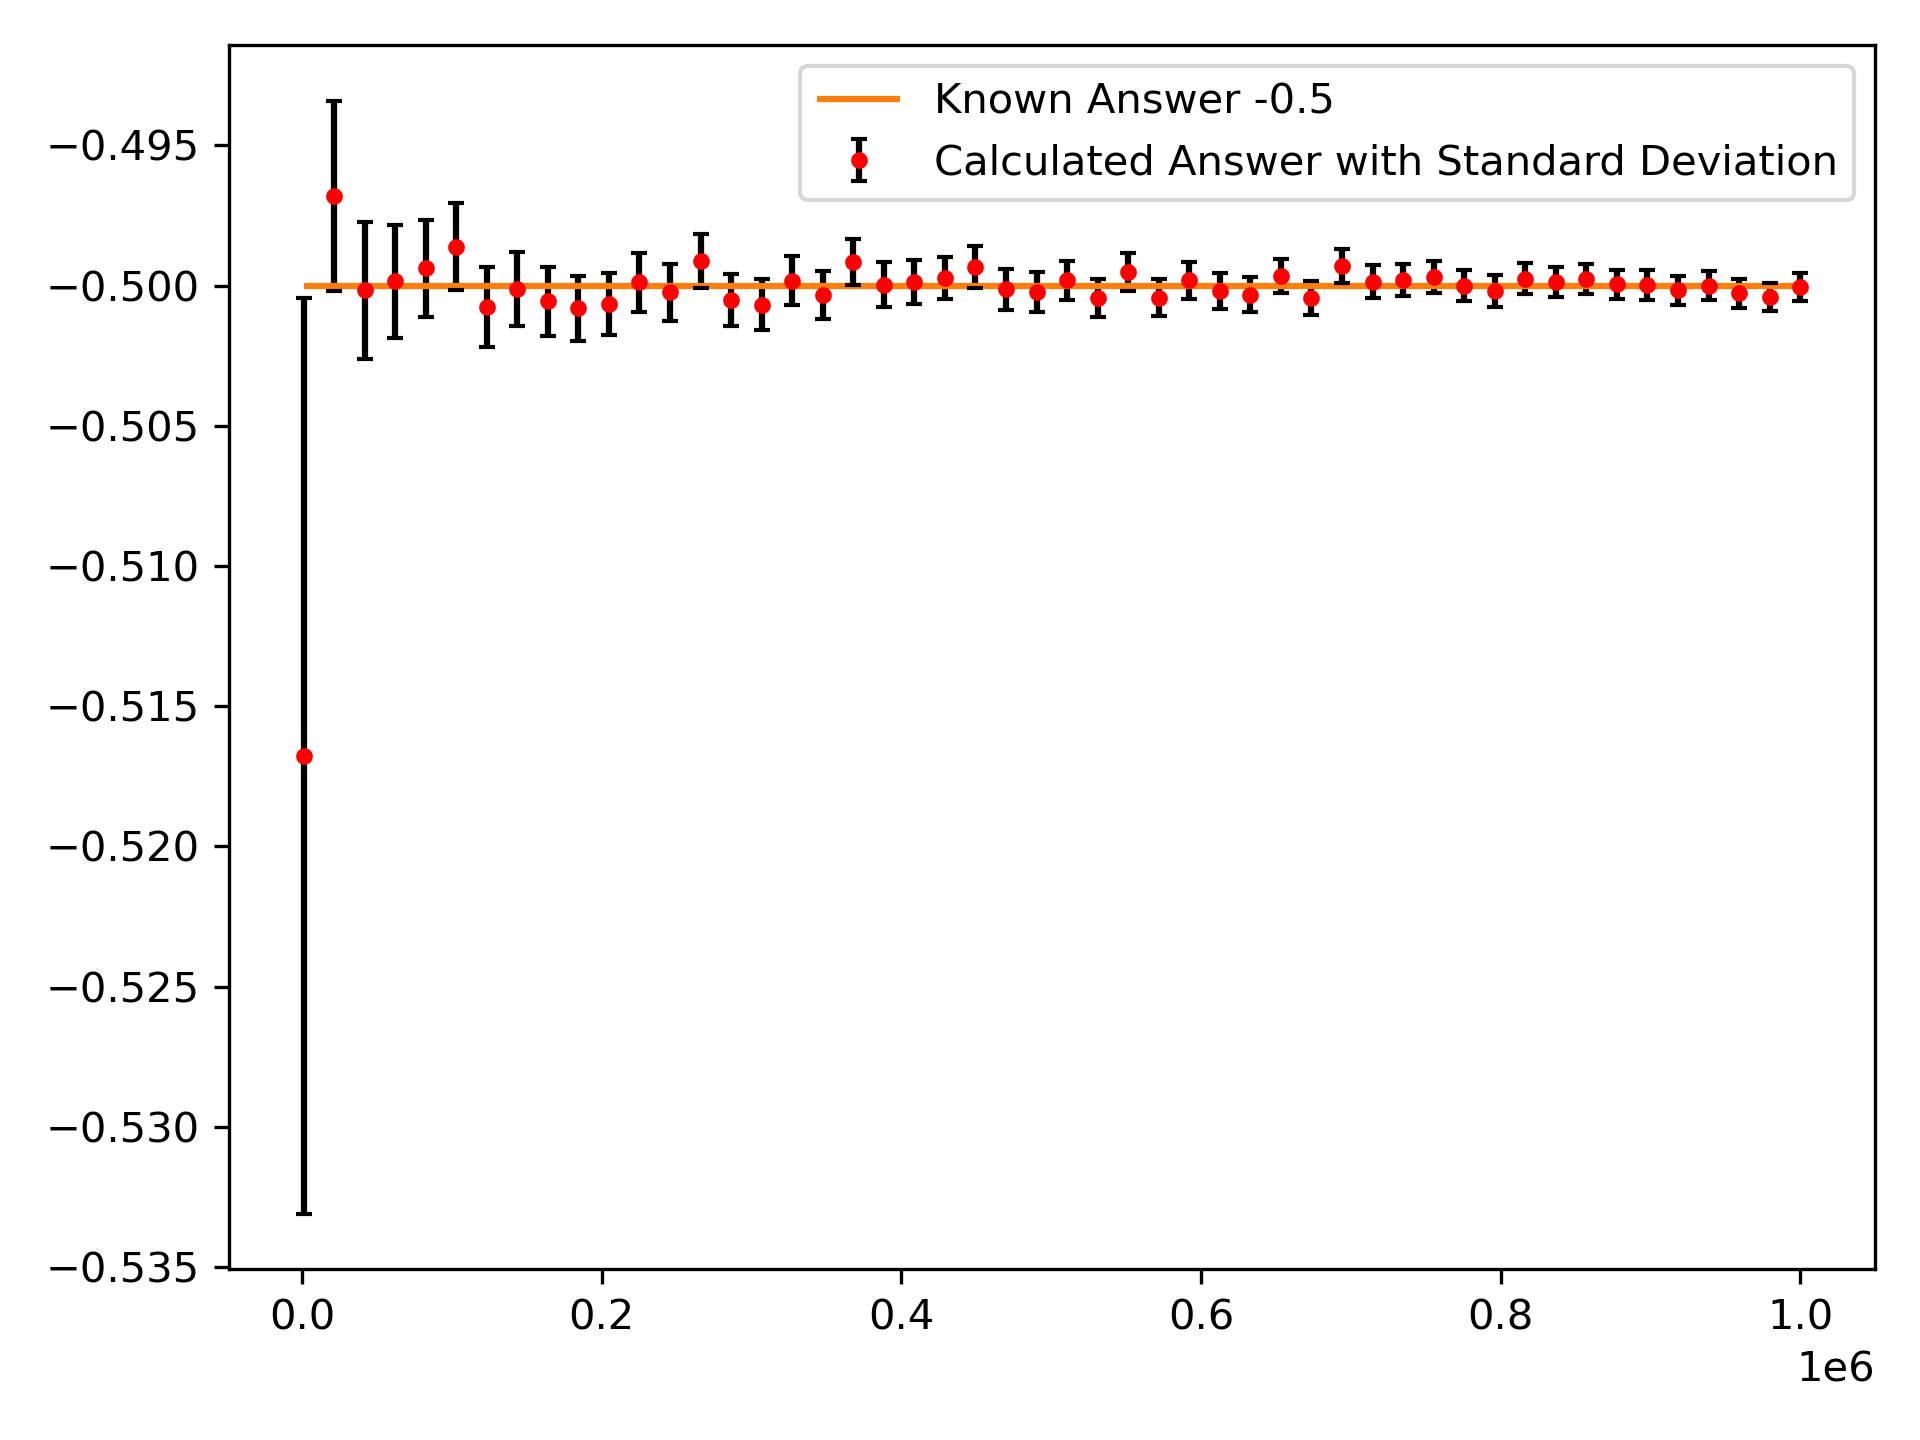
\includegraphics[width=0.7\textwidth]{task_2_b.png}
  \end{center}
  \caption{Plot showing the convergence of calculated guesses over a range of N random points (from $10^3$ to $10^6$)}
  \label{fig:task_2_b}
\end{figure}


% subsection subsection name (end)

\subsection{Part c} % (fold)
\label{sub:Part c}


Integral output (to a 90\% confidence) = [5.336] $\pm$  2.19e-06 units.
\\
Sample Size = [1e+06].
\\
Time Taken = [0.512]s.
\\
Variance = [1.78].
\\
Root-Mean-Square = [1.79].
\\
Standard Deviation (Of Distribution/X-axis) = [0.00133]/[1.33].

\vspace{1em}

For part c of task 2 the function $f(x)=x^2$ is similarly as easy to 
integrate with the largest deviating point on figure \ref{fig:task_2_c} 
being $\approx 1\%$ off.

\begin{figure}[H]
  \begin{center}
    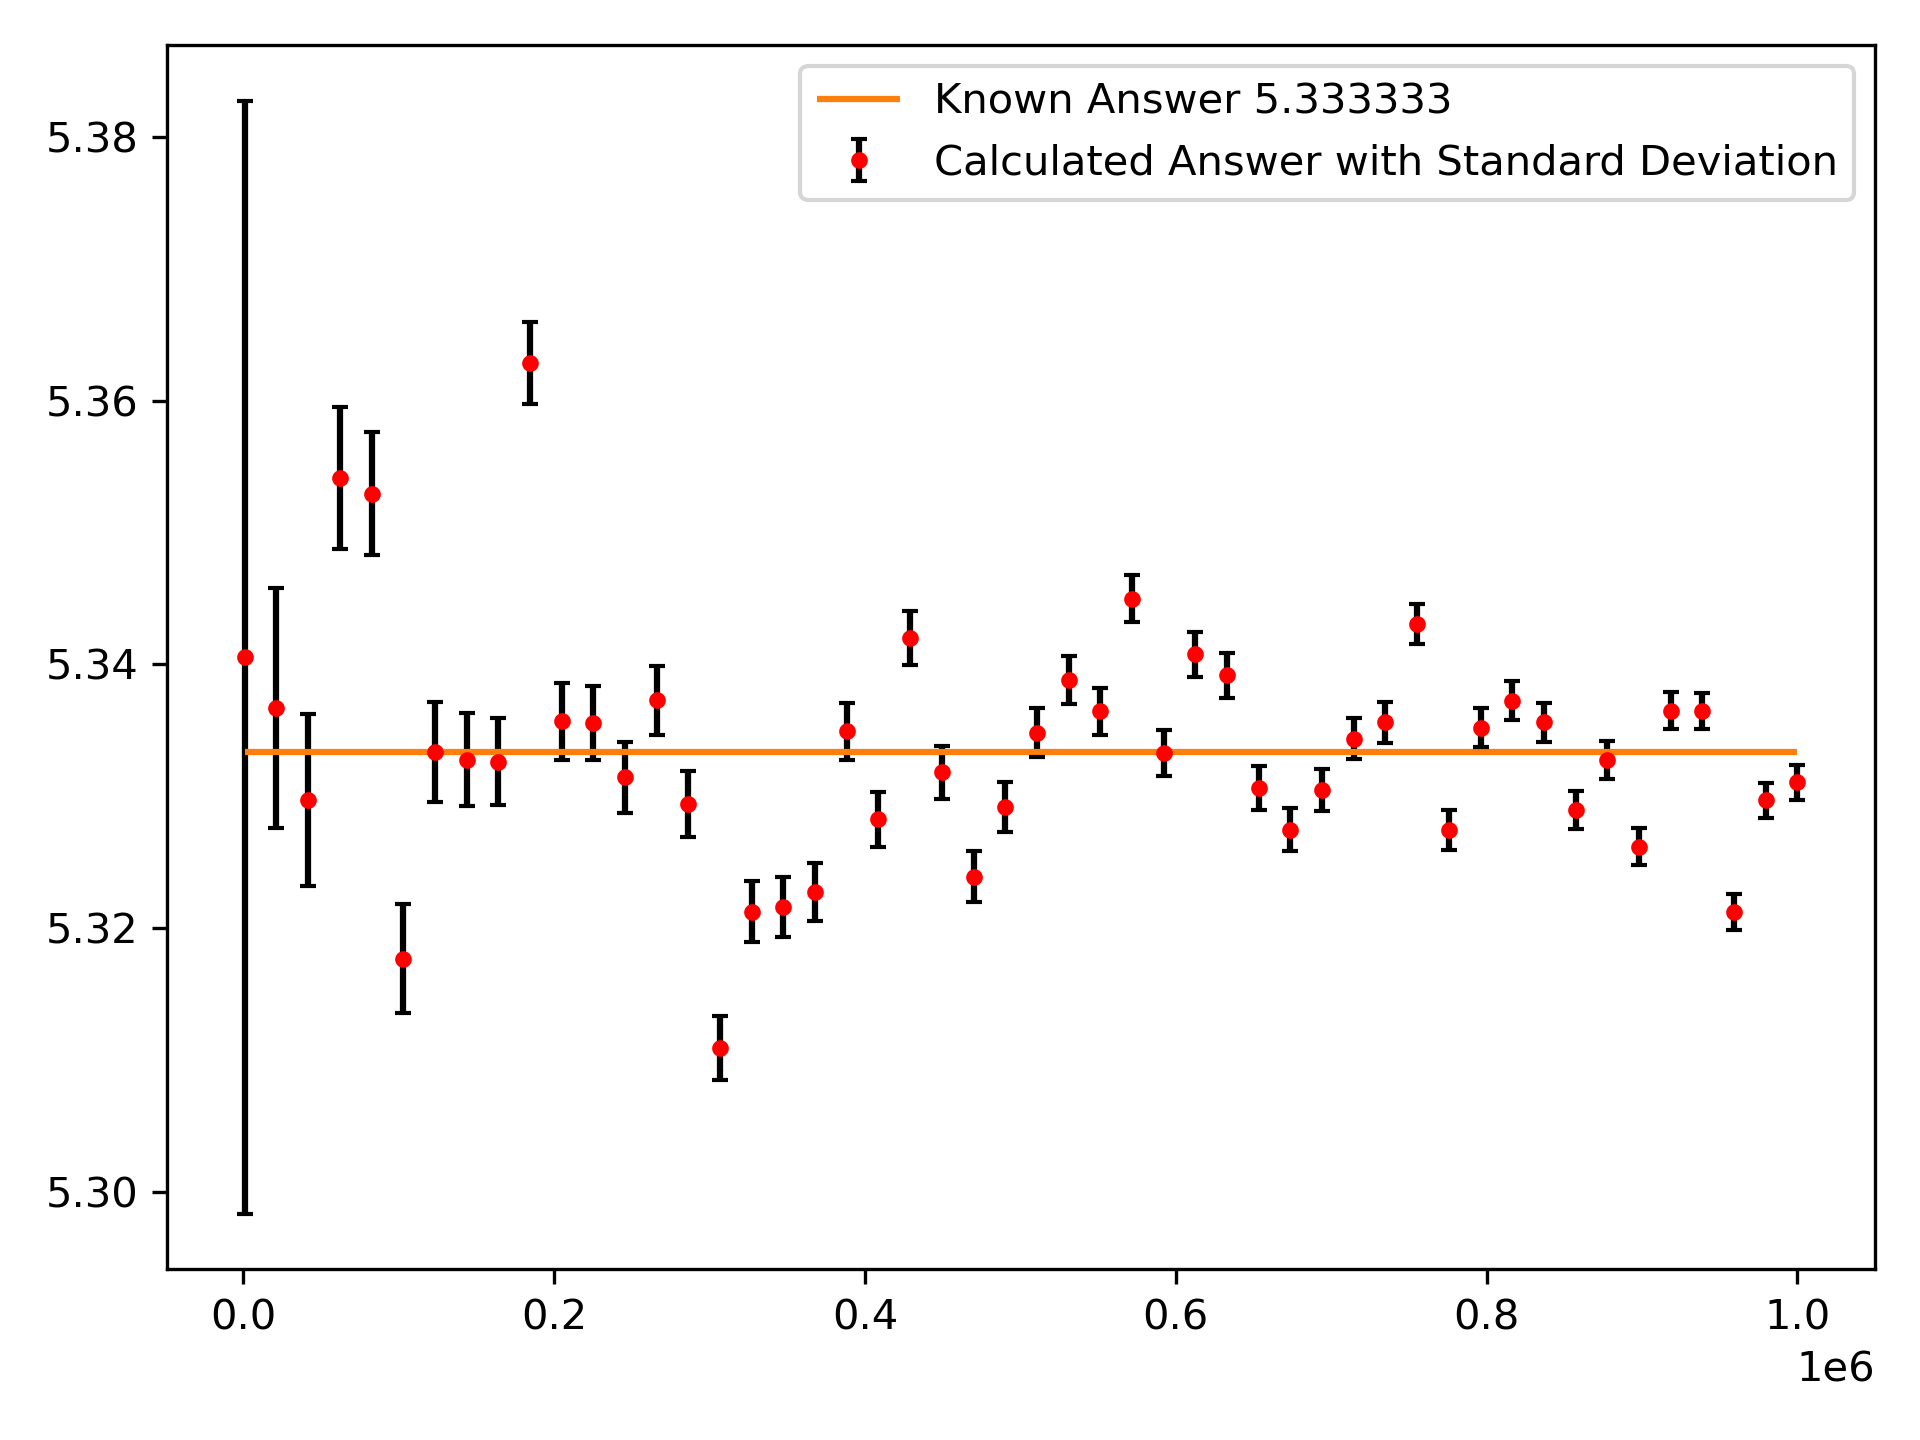
\includegraphics[width=0.7\textwidth]{task_2_c.png}
  \end{center}
  \caption{Plot showing the convergence of calculated guesses over a range of N random points (from $10^3$ to $10^6$)}
  \label{fig:task_2_c}
\end{figure}


% section section name (end)

\subsection{Part d} % (fold)
\label{sub:Part d}


Integral output (to a 90\% confidence) = [0.75] $\pm$  1.23e-06 units.
\\
Sample Size = [1e+06].
\\
Time Taken = [0.466]s.
\\
Variance = [0.563].
\\
Root-Mean-Square = [0.882].
\\
Standard Deviation (Of Distribution/X-axis) = [0.00075]/[0.75].

\vspace{1em}

For part d of task 2 the function $f(x,y)=xy+y$ was again trivial to calculate 
with the furthest point on figure \ref{fig:task_2_d} being $\approx 2\%$ off of the known 
answer. 

\begin{figure}[H]
  \begin{center}
    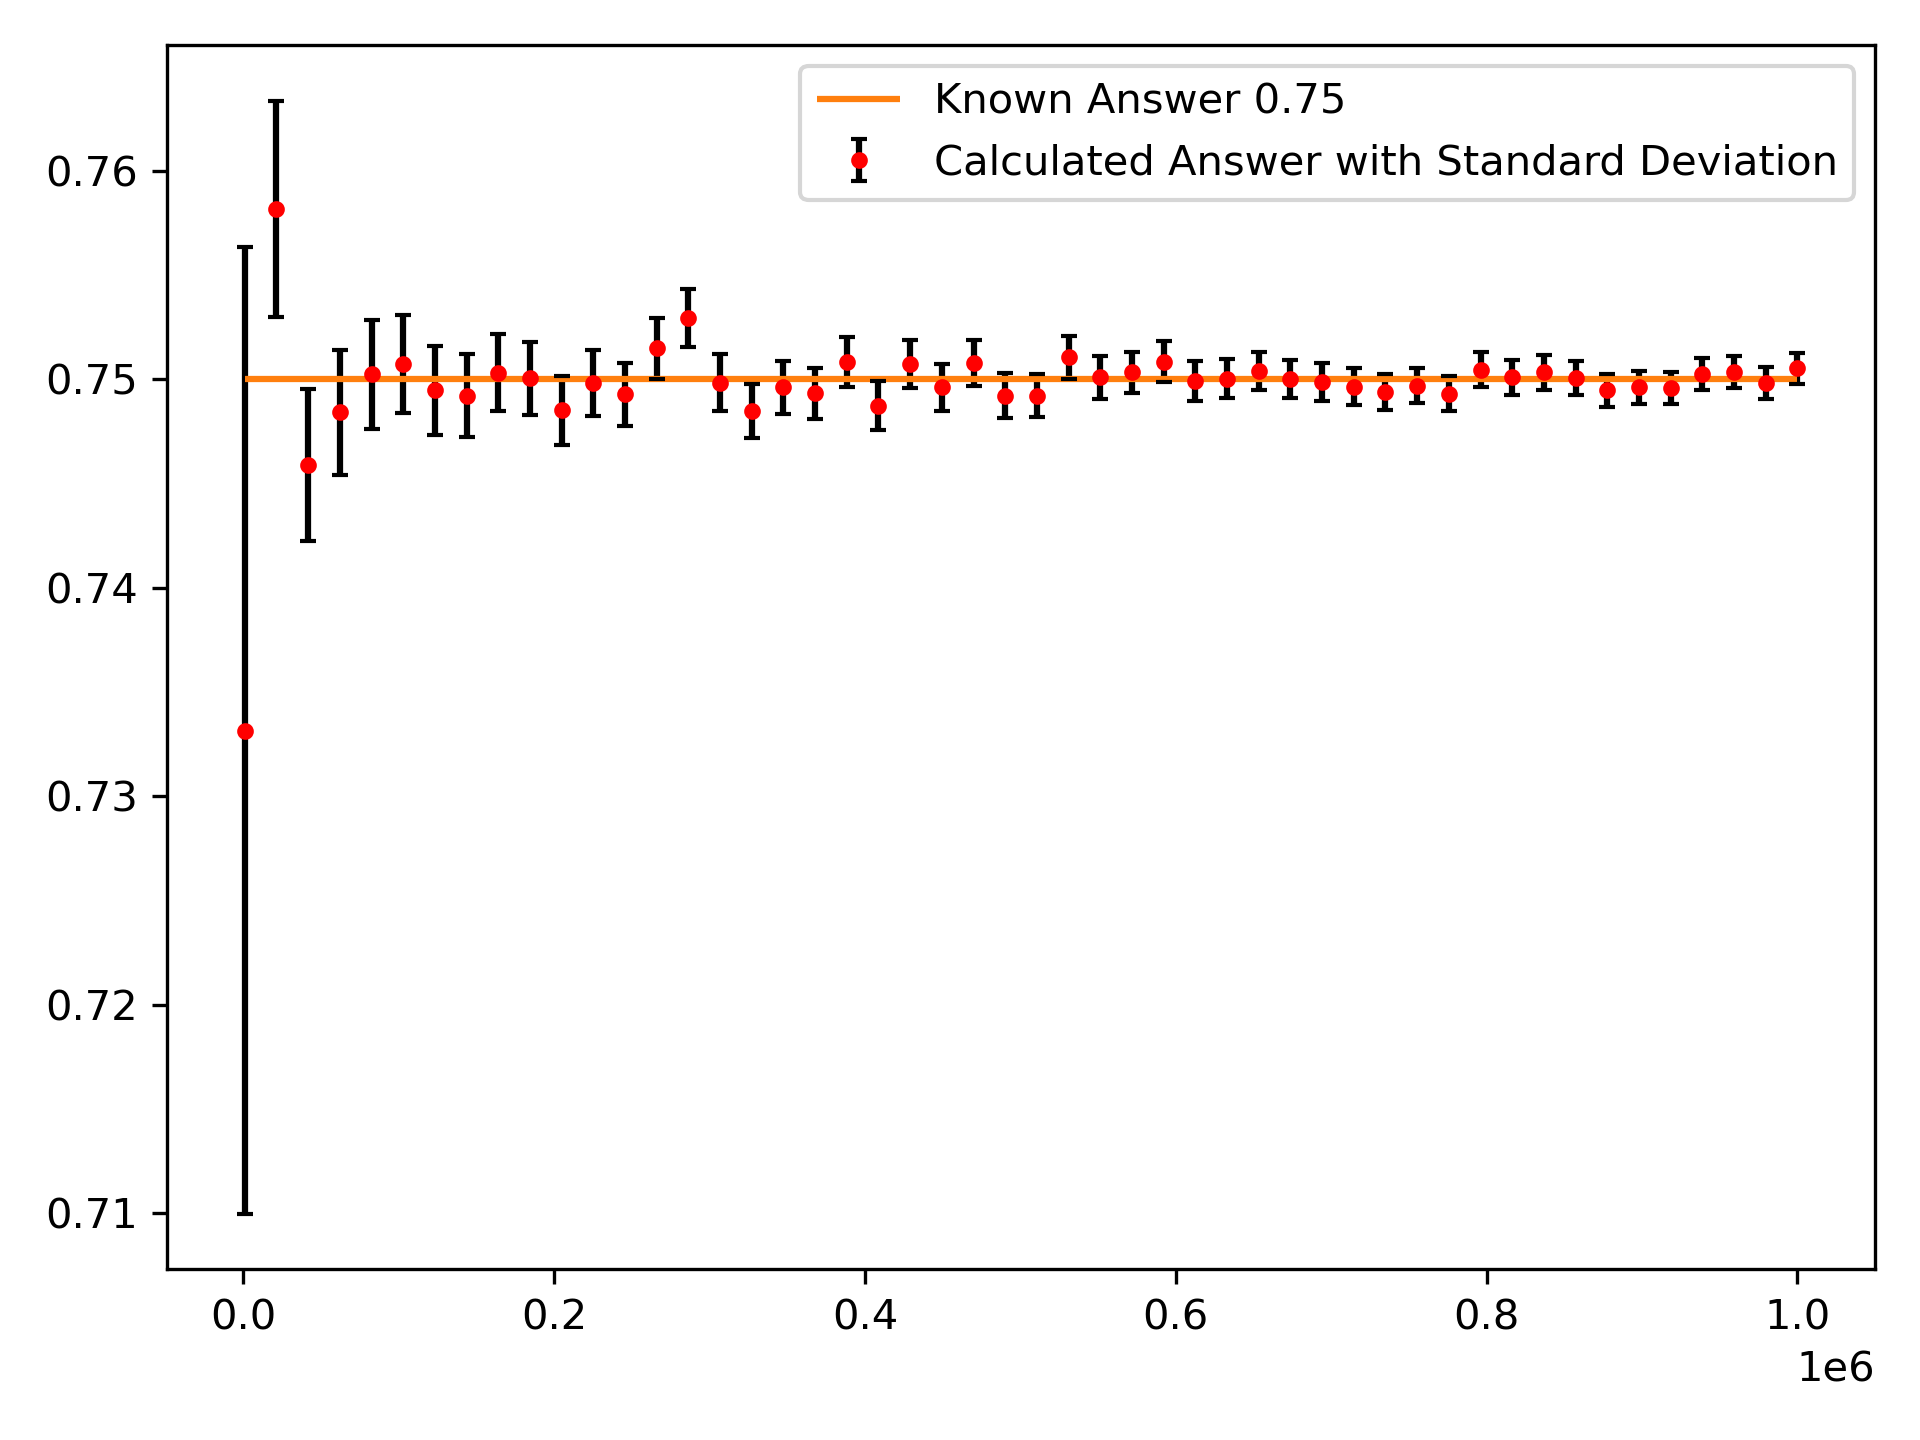
\includegraphics[width=0.7\textwidth]{task_2_d.png}
  \end{center}
  \caption{Plot showing the convergence of calculated guesses over a range of N random points (from $10^3$ to $10^6$)}
  \label{fig:task_2_d}
\end{figure}

\section{Task 3} % (fold)
\label{sec:Task 3}

Use your subroutine to evaluate the size of the region enclosed
within an n-sphere of radius 2.0, for n = 3 (i.e. the volume of a ball of
radius 1.5) and n = 5.

\subsection{Result for r = 2 \& n = 3} % (fold)
\label{sub:Result for r = 2}

% subsection subsection name (end)

Integral output (to a 90\% confidence) = [33.48] $\pm$  8.61e-07 units.
\\
Sample Size = [1e+06].
\\
Time Taken = [0.561]s.
\\
Variance = [0.274].
\\
Root-Mean-Square = [0.723].
\\
Standard Deviation (Of Distribution/X-axis) = [0.000523]/[0.523].

\vspace{1em}

For task 3 the same Monte-Carlo method was used but in addition with another
function. This function counted all the points that were inside the circle and divided that by 
the number of total points, then this was multiplied by the area which the circle 
was in, producing the relative area. From figure \ref{fig:task_3_n3} it can be seen that 
the method converges up until a point and then varies around the answer.

\begin{figure}[H]
  \begin{center}
    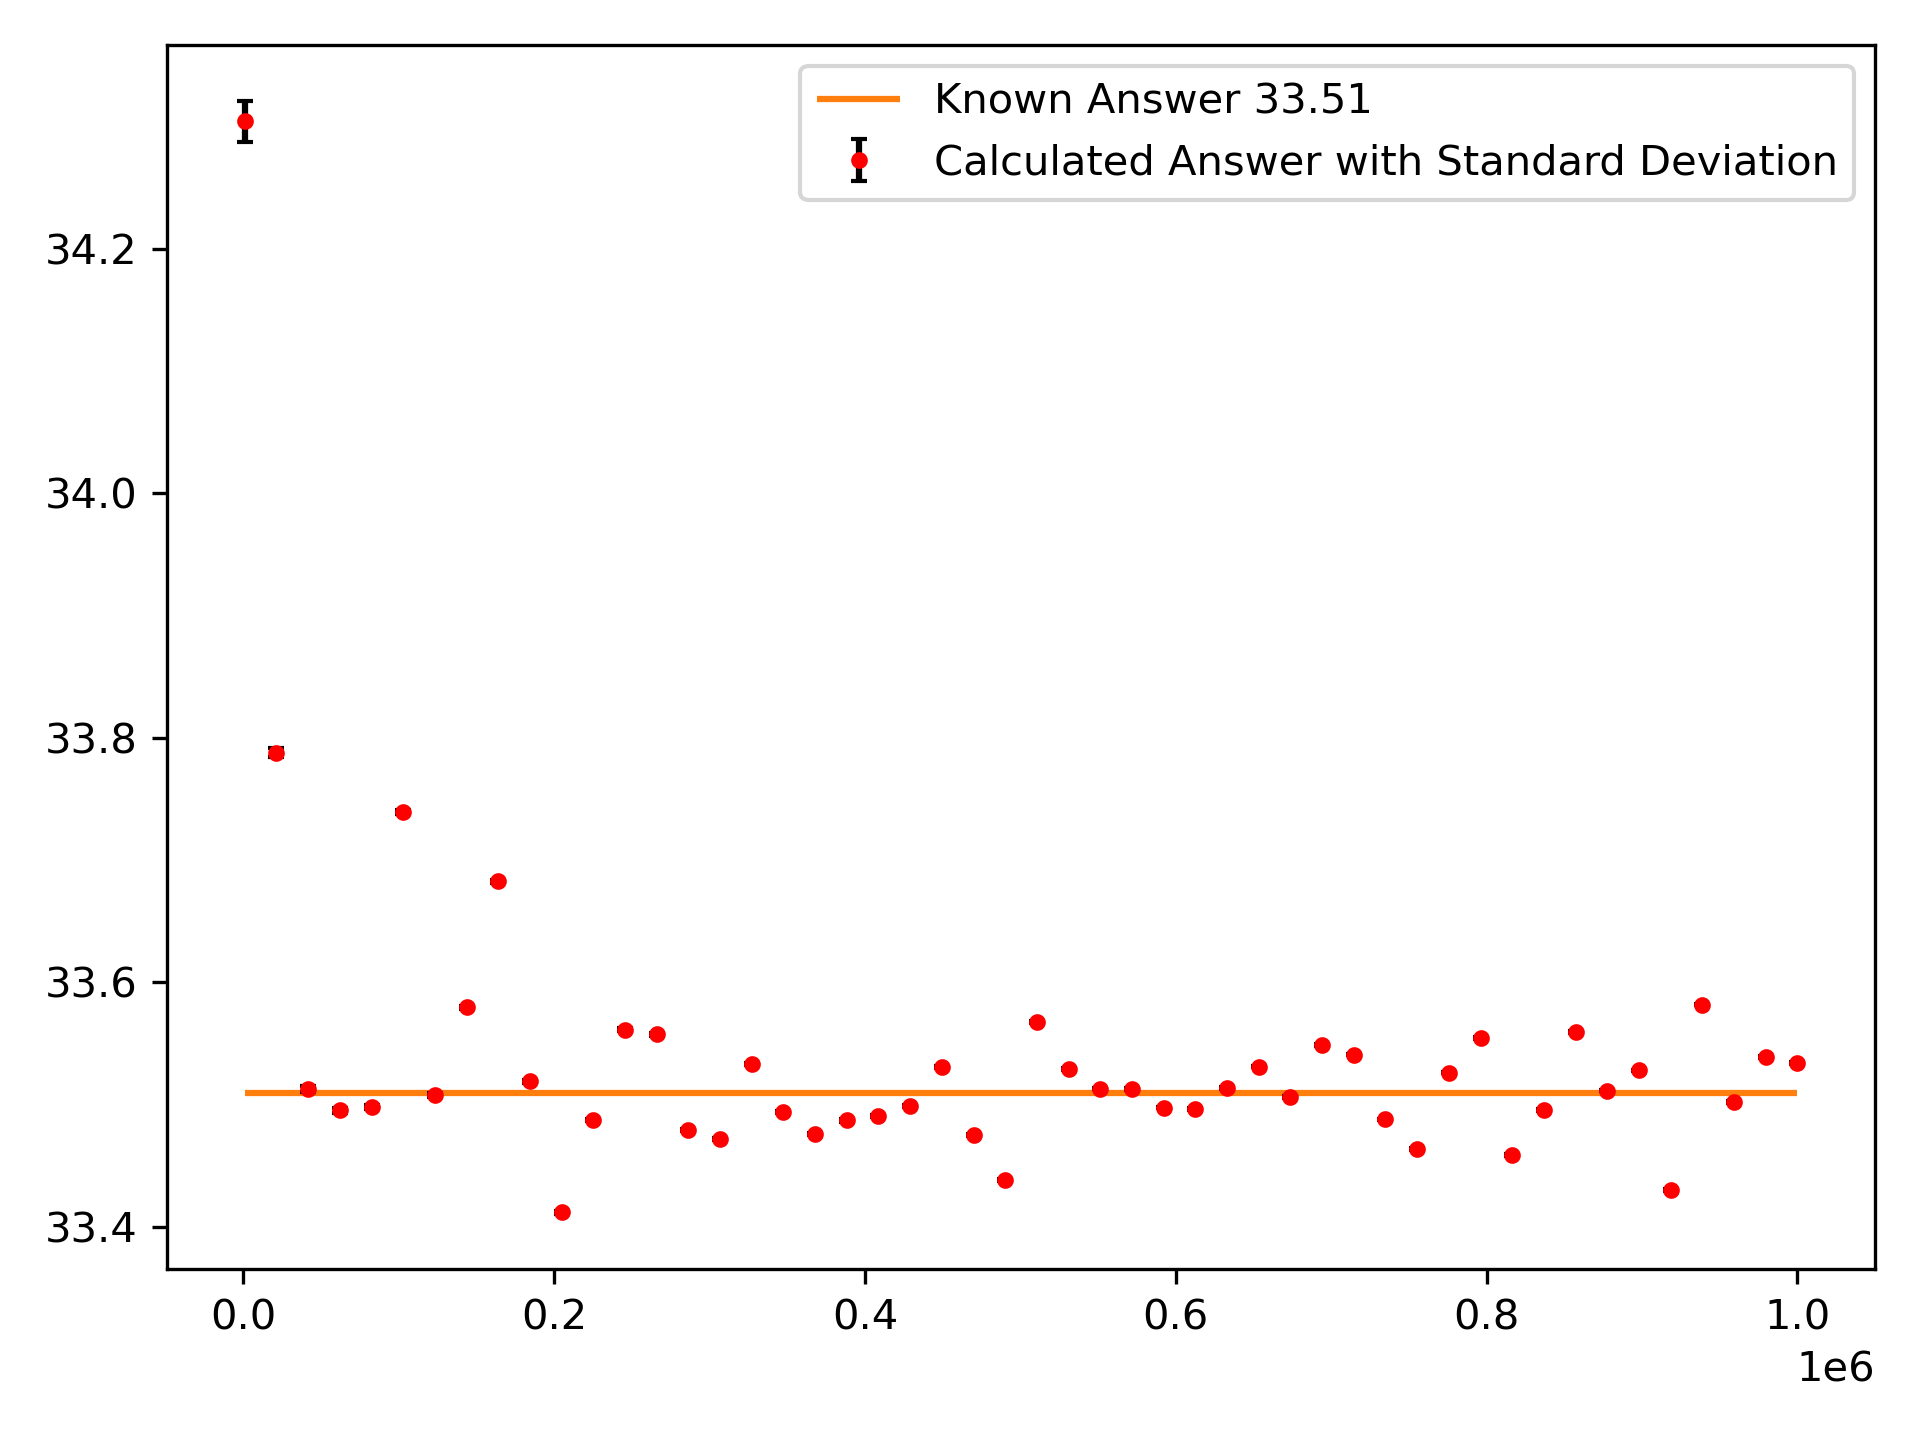
\includegraphics[width=0.7\textwidth]{task_3_n3.png}
  \end{center}
  \caption{Plot showing the convergence of calculated guesses over a range of N random points (from $10^3$ to $10^6$)}
  \label{fig:task_3_n3}
\end{figure}


% section section name (end)

\subsection{Result for r = 1.5 \& n = 5} % (fold)
\label{sub:Result for r = 1.5}

Integral output (to a 90\% confidence) = [40.13] $\pm$  6.45e-08 units.
\\
Sample Size = [1e+06].
\\
Time Taken = [0.551]s.
\\
Variance = [0.00154].
\\
Root-Mean-Square = [0.198].
\\
Standard Deviation (Of Distribution/X-axis) = [3.92e-05]/[0.0392]. 

\vspace{1em} 

As mentioned in the notes this isn't a good method to use for the integration 
of hypersphere's and that can be seen in one of the low sample points ($10^3$) on 
figure \ref{fig:task_3_n5} being $\approx 30\%$ off. Like the last figure (\ref{fig:task_3_n3}) 
the Monte-Carlo method seems to vary around the correct answer without much improvement.

\begin{figure}[H]
  \begin{center}
    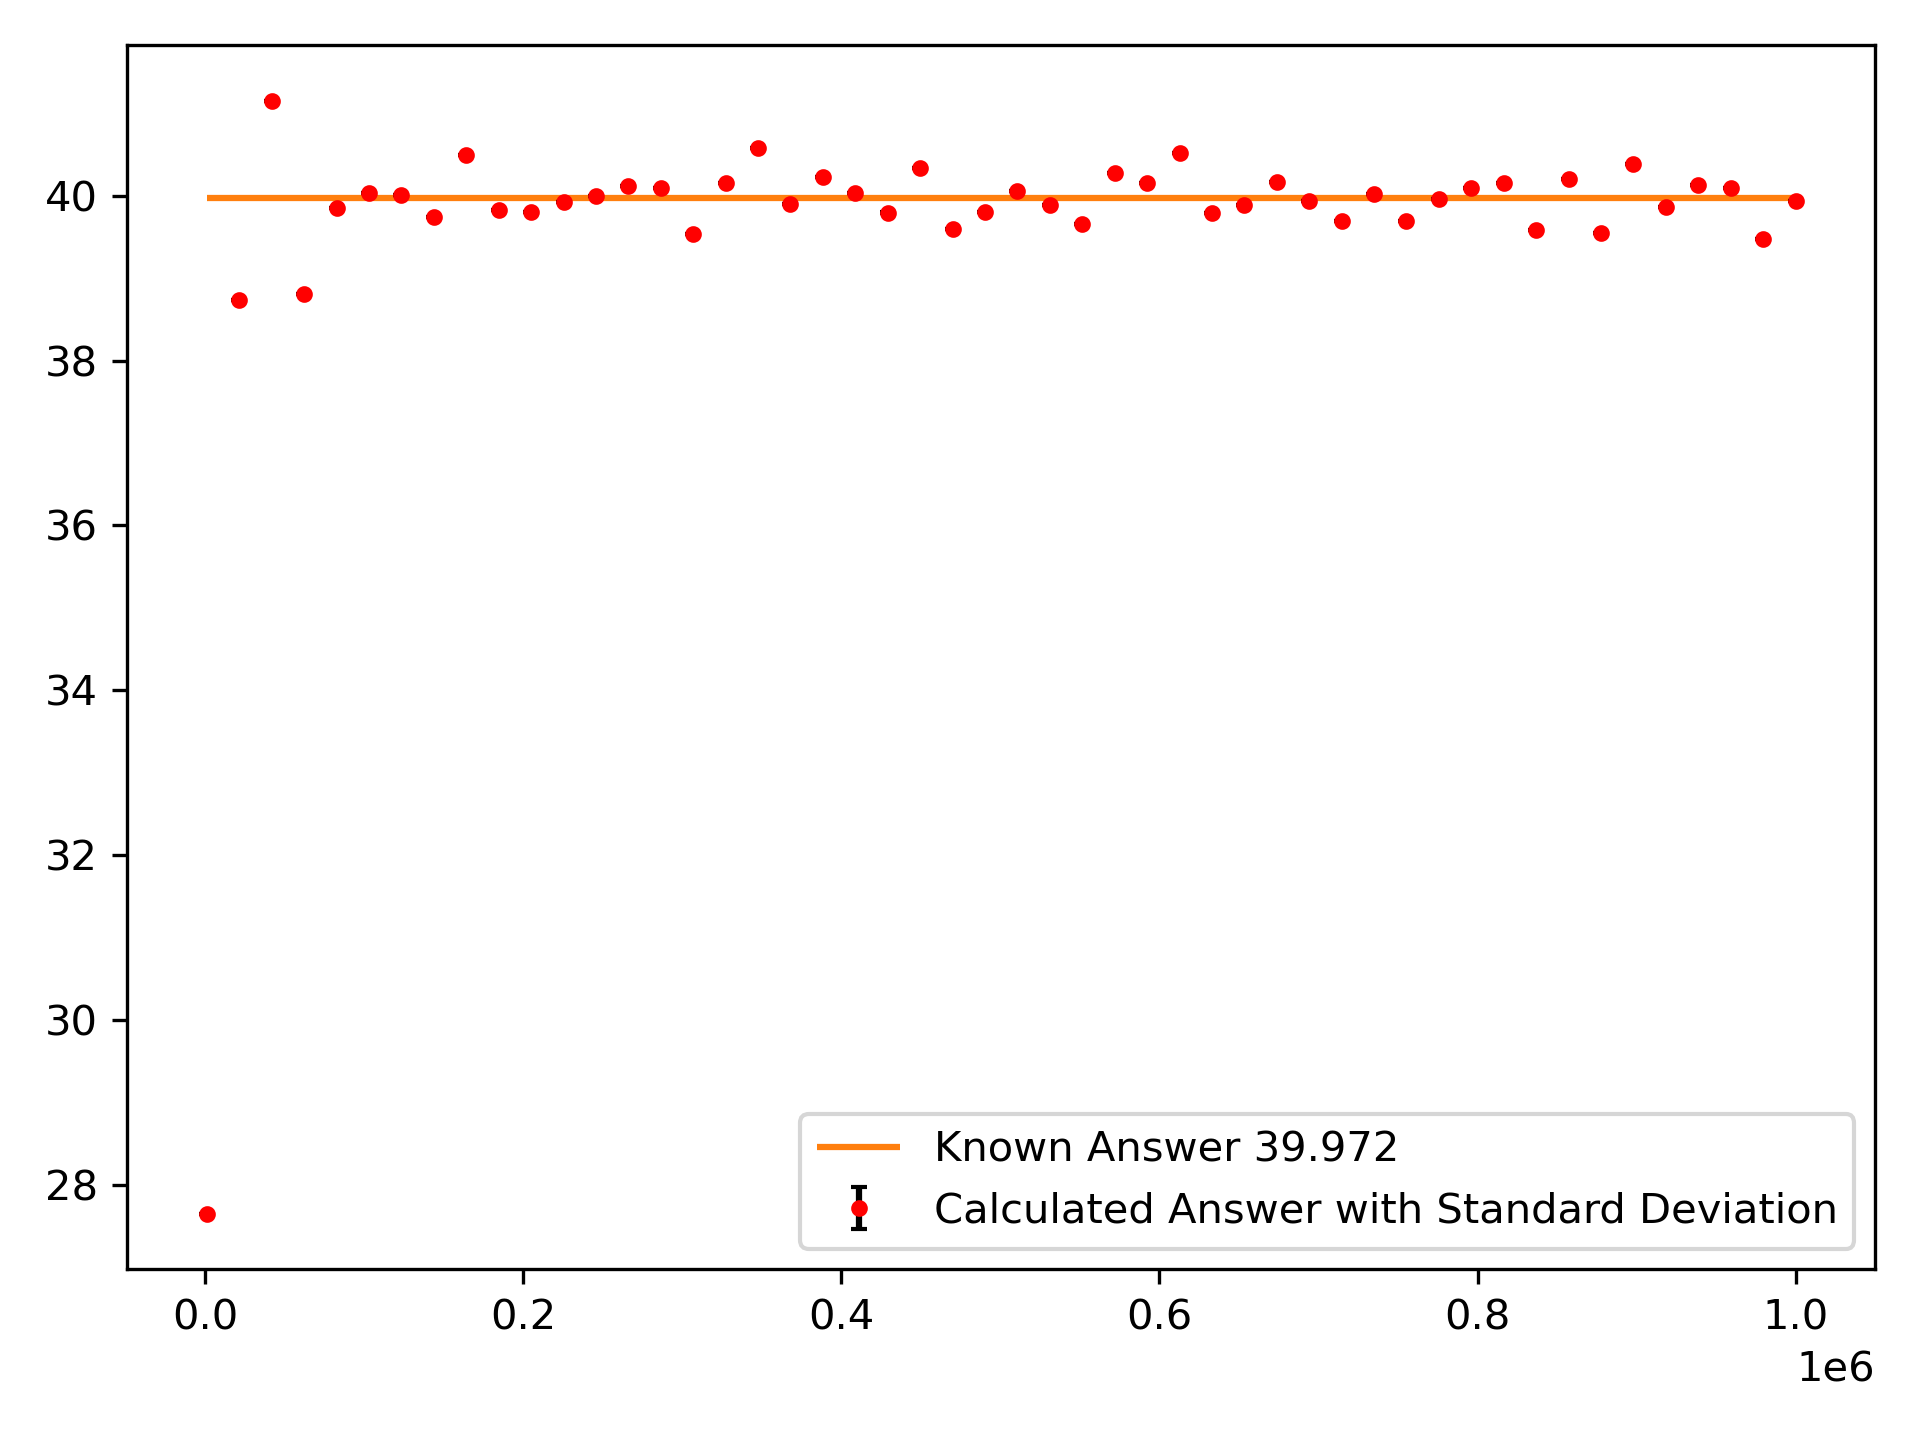
\includegraphics[width=0.7\textwidth]{task_3_n5.png}
  \end{center}
  \caption{Plot showing the convergence of calculated guesses over a range of N random points (from $10^3$ to $10^6$)}
  \label{fig:task_3_n5}
\end{figure}

% subsection subsection name (end)

\section{Task 4} % (fold)
\label{sec:Task 4}

% section section name (end)

% subsection subsection name (end)
\section{Task 5} % (fold)
\label{sec:Task 5}


Implement new code to apply importance sampling to evaluate one
dimensional integrals. Use the Metropolis method to generate the
non-uniform random sampling of the weighting function (and
remember that the weighting function must be normalised correctly ).
Use this new function to evaluate the definite integrals

$$a) \int^{+10}_{-10}2e^{-x^2}dx \;\; \textrm{using } e^{-|x|} \;\; \textrm{as the sampling function}$$

$$b) \int^{\pi}_{0}1.5\cdot \sin(x) dx \;\; \textrm{noting that } \sin(x)\approx \frac{4}{\pi^2}\cdot x \cdot (\pi - x) \;\; \textrm{in this region}$$


\subsection{Part a} % (fold)
\label{sub:task5Parta}

Integral output (to a 90\% confidence) = [3.542] $\pm$  5.57e-07 units.
\\
Sample Size = [1e+05].
\\
Time Taken = [1.29]s.
\\
Variance = [-0.00115].
\\
Root-Mean-Square = [1.41].
\\
Standard Deviation (Of Distribution/X-axis) = [0.000107]/[0.0339]. 

\vspace{1em}

In Task 5 the importance sapling and Metropolis method were employed to make the 
integration of functions more efficient, this is done by having a sampling function that the Metropolis
method draws a set of non-uniform set of random samples from. As can be seen in figure \ref{fig:task_5_a},
apart from the initial point in which it only has one sample, the range of samples converges immediately.

\begin{figure}[H]
  \begin{center}
    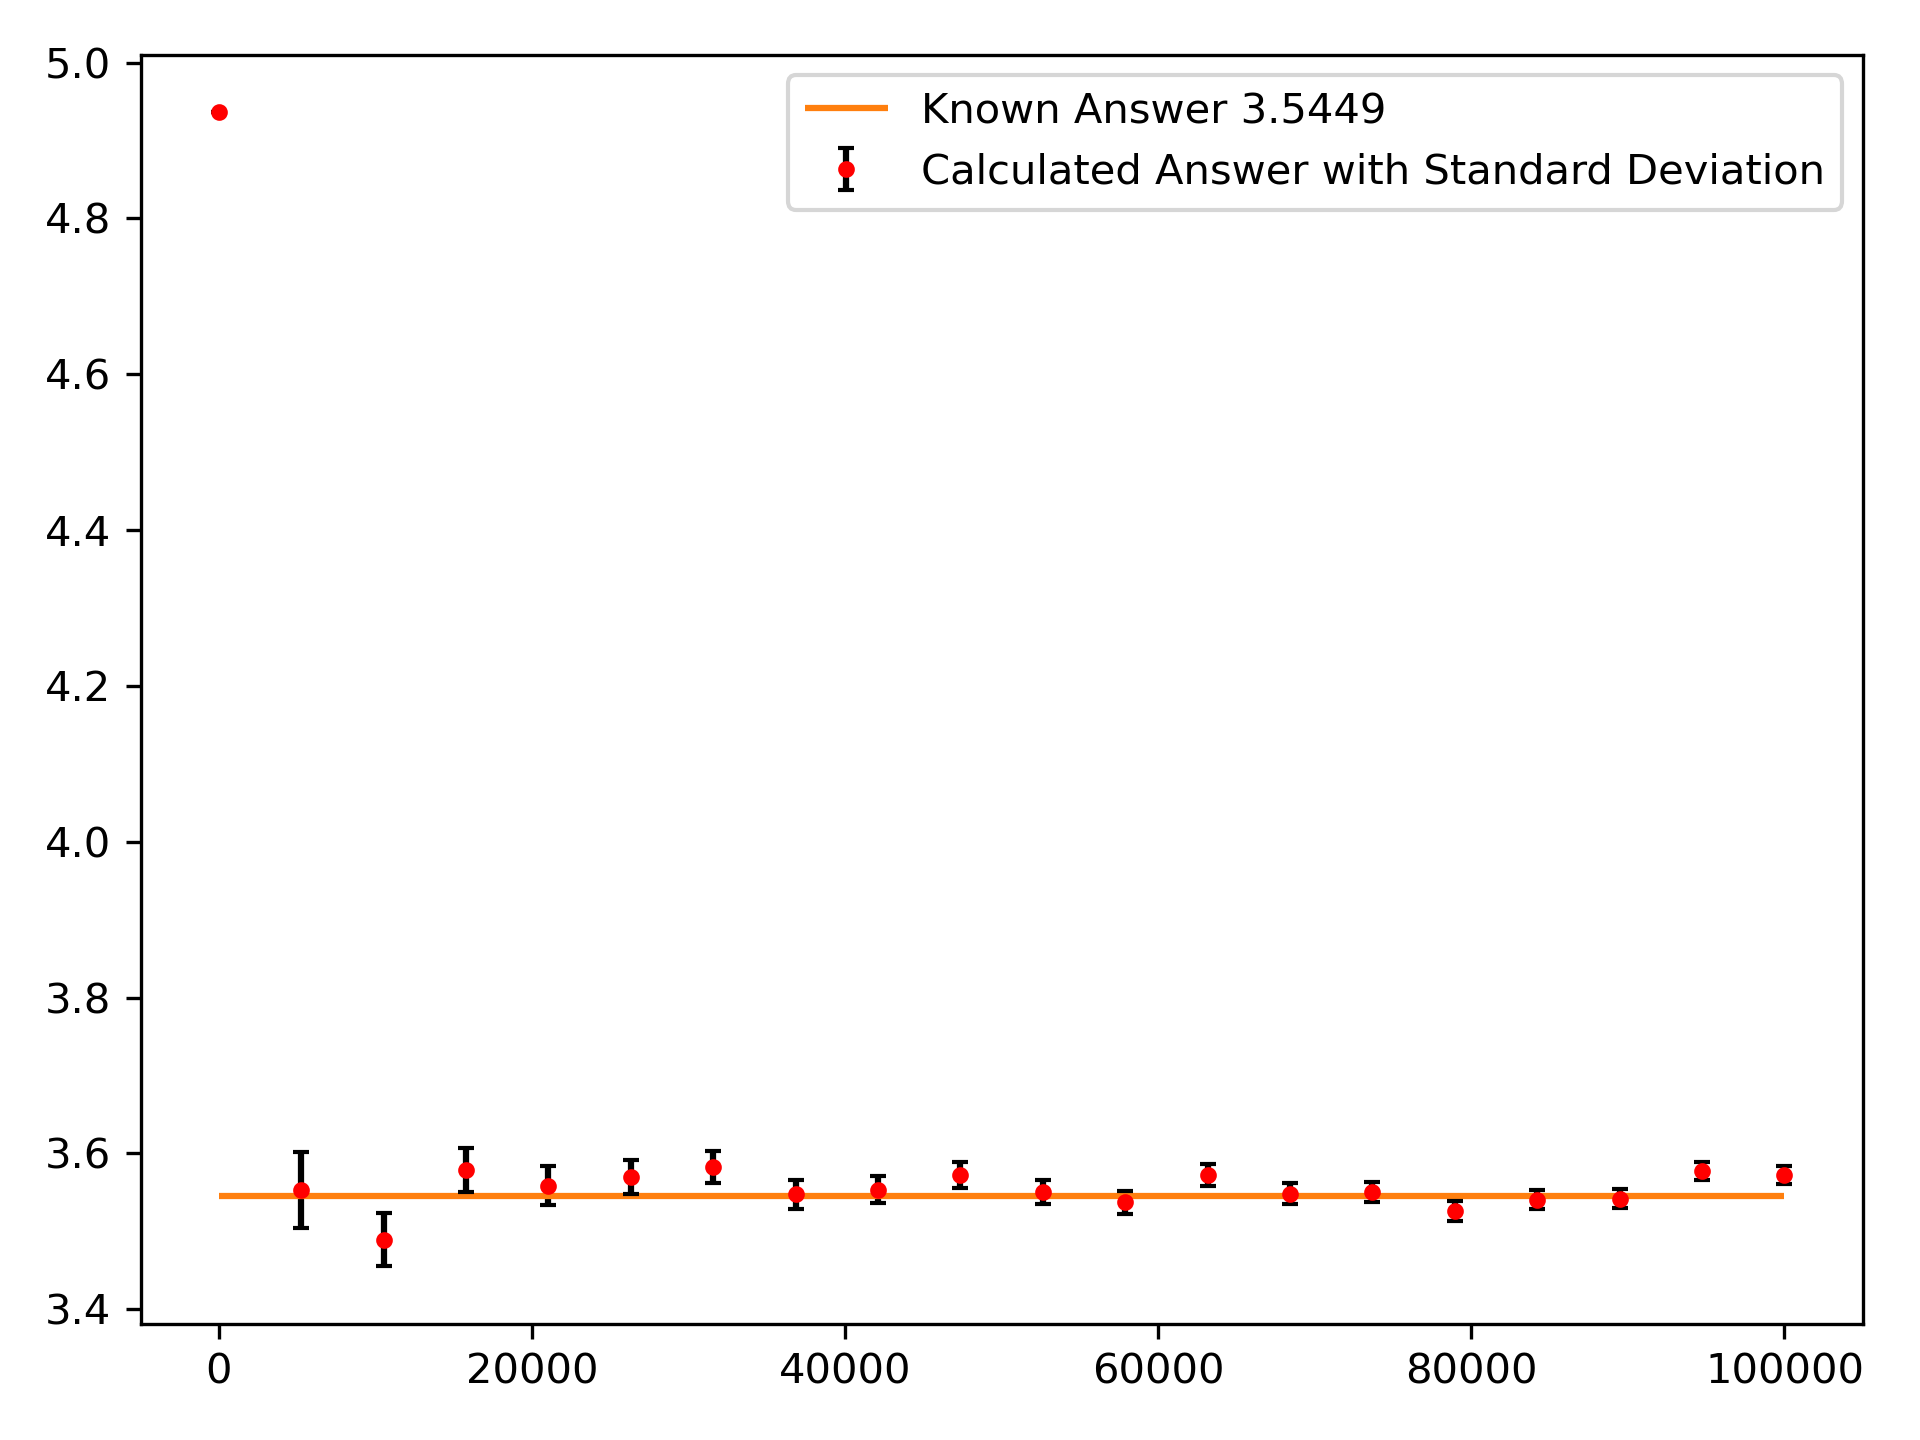
\includegraphics[width=0.7\textwidth]{task_5_a.png}
  \end{center}
  \caption{Plot showing the convergence of calculated guesses over a range of N random points (from $1$ to $10^5$)}
  \label{fig:task_5_a}
\end{figure}


\subsection{Part b} % (fold)
\label{sub:task5Part b}

Integral output (to a 90\% confidence) = [3.0] $\pm$  4.93e-05 units.
\\
Sample Size = [1e+05].
\\
Time Taken = [1.06]s.
\\
Variance = [-9.0].
\\
Root-Mean-Square = [3.0].
\\
Standard Deviation (Of Distribution/X-axis) = [0.00949]/[3.0]. 


\vspace{1em}

In part b of task 5 again pretty much all the amounts of different points converge 
to the answer immediately.

\begin{figure}[H]
  \begin{center}
    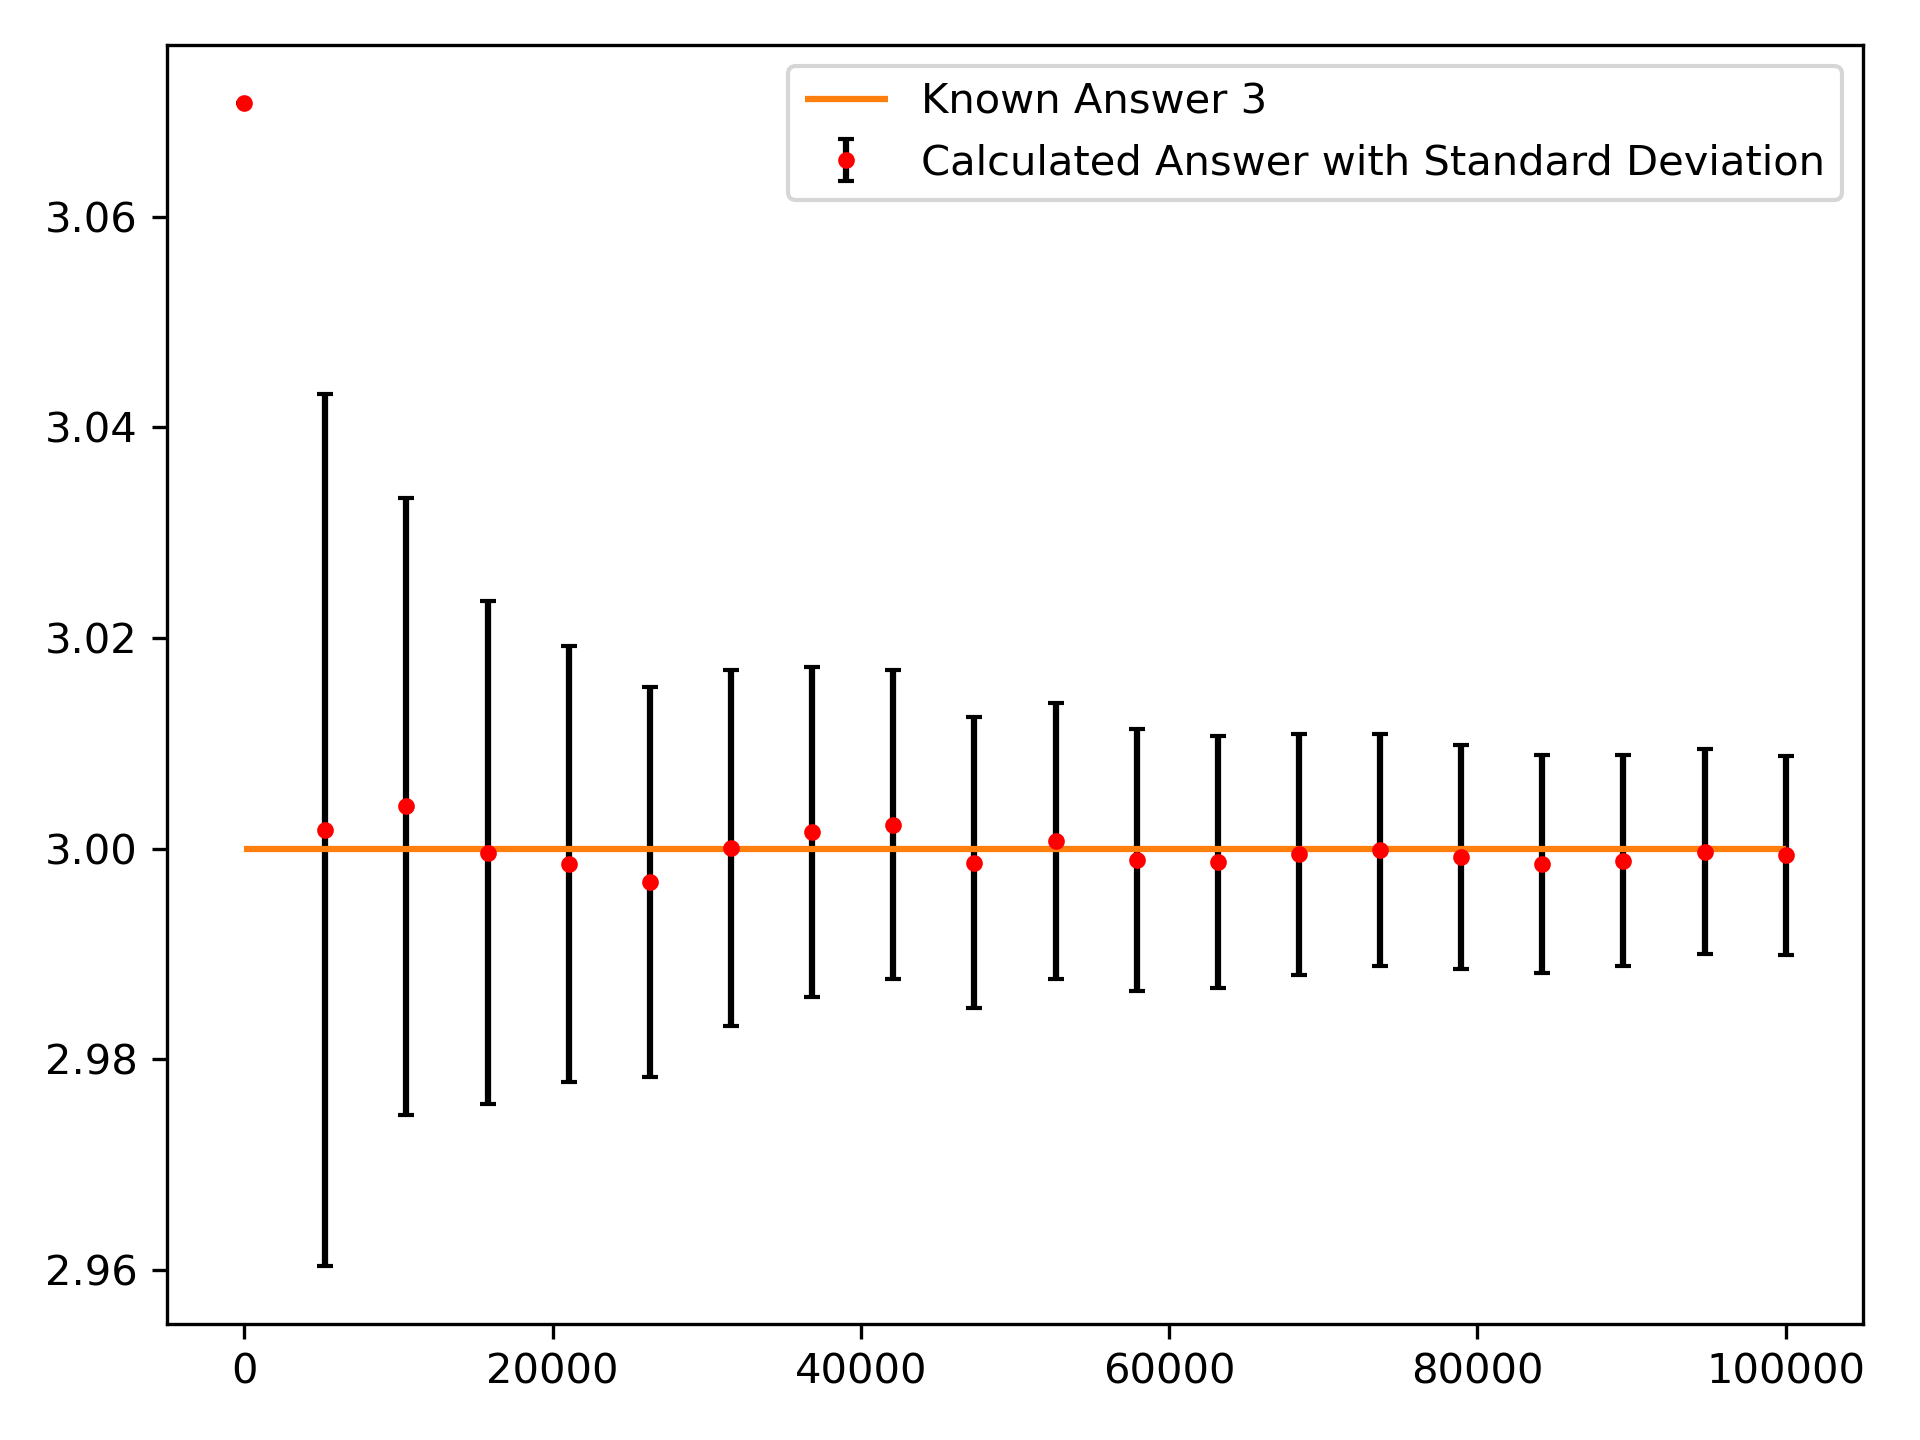
\includegraphics[width=0.7\textwidth]{task_5_b.png}
  \end{center}
  \caption{Plot showing the convergence of calculated guesses over a range of N random points (from $1$ to $10^5$)}
  \label{fig:task_5_b}
\end{figure}

\section{Task 6} % (fold)
\label{sec:Task 6}

Evaluate both integrals in task 5 with uniform sampling – Compare
your importance sampled result with the answer obtained using
uniform sampling. You should compare and contrast the number of
points required to achieve an answer of equal accuracy using the
two methods.

\subsection{Part a} % (fold)
\label{sub:6Part a}

Integral output (to a 90\% confidence) = [3.581] $\pm$  2.95e-06 units.
\\
Sample Size = [1e+05].
\\
Time Taken = [0.225]s.
\\
Variance = [0.0321].
\\
Root-Mean-Square = [0.505].
\\
Standard Deviation (Of Distribution/X-axis) = [0.000566]/[0.179]. 

\vspace{1em}

Task 6 is comparing the uniform sampling method with the importance sampled method. 
In part a the importance sampled method obtained a result of $3.542 \pm 5.57e-07$ that took 
approximately 1.29 seconds, and had a variance of 0.00115. The uniform sampled method got a result 
of $3.581 \pm 2.95e-06$ that took 0.225 seconds and had a variance of 0.0321. The importance sampled 
method is 0.08\% off while the uniform method is 1\% off, that makes it $\approx 12x$ more accurate. 
This is a worth while method to use if accuracy is extremely important and for speed since the 
uniform method is only $\approx 6x$ faster, although time does have to be spent 
setting up the sampled function.

\begin{figure}[H]
  \begin{center}
    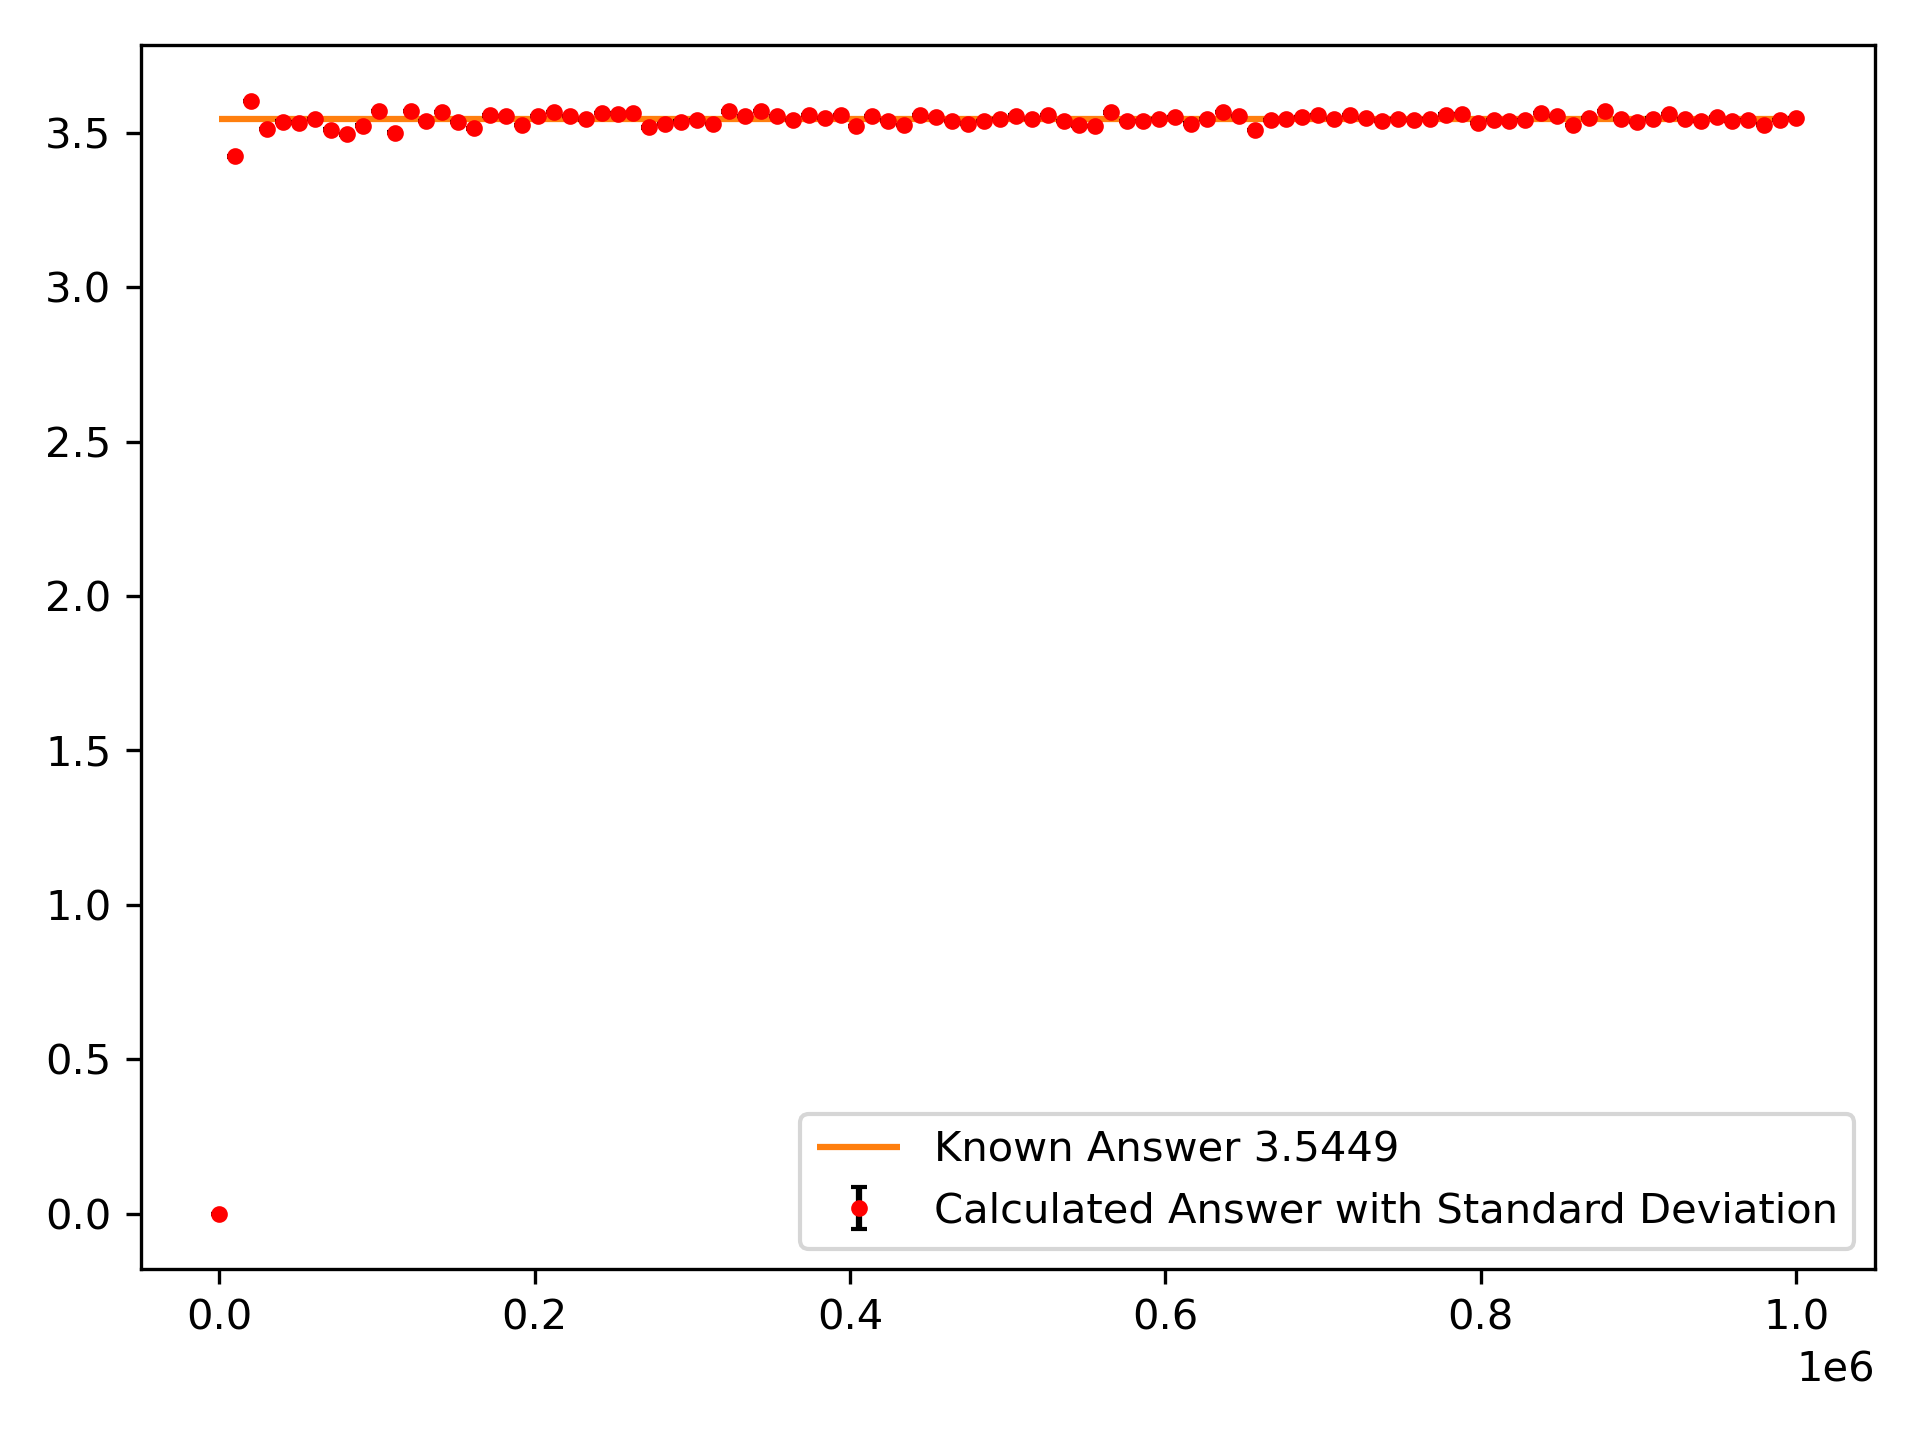
\includegraphics[width=0.7\textwidth]{task_6_a.png}
  \end{center}
  \caption{Plot showing the convergence of calculated guesses over a range of N random points (from $1$ to $10^6$)}
  \label{fig:task_6_a}
\end{figure}


\subsection{Part b} % (fold)
\label{sub:6Part b} 

Integral output (to a 90\% confidence) = [3.007] $\pm$  1.57e-05 units.
\\
Sample Size = [1e+05].
\\
Time Taken = [0.135]s.
\\
Variance = [0.916].
\\
Root-Mean-Square = [1.06].
\\
Standard Deviation (Of Distribution/X-axis) = [0.00303]/[0.957]. 

\vspace{1em}

Comparing both part b's the importance sampled method obtained a result of $3.04 \pm 2.58e-05$ that took 
approximately 1.06 seconds, and had a variance of 0.00115. The uniform sampled method got a result 
of $3.007 \pm 1.57e-05$ that took 0.135 seconds and had a variance of 0.916. As can be seen in figures 
\ref{fig:task_5_a},\ref{fig:task_5_b},\ref{fig:task_6_a} and \ref{fig:task_6_b} the convergence rate of 
each method from a range of points that vary from $1$ to $10^5$ random numbers are all similar, the main 
factor that distinguishes them is the variance. This makes sense since the sampled functions are approaching 
being flat, which would be more consistently filled by a range of random numbers.

\begin{figure}[H]
  \begin{center}
    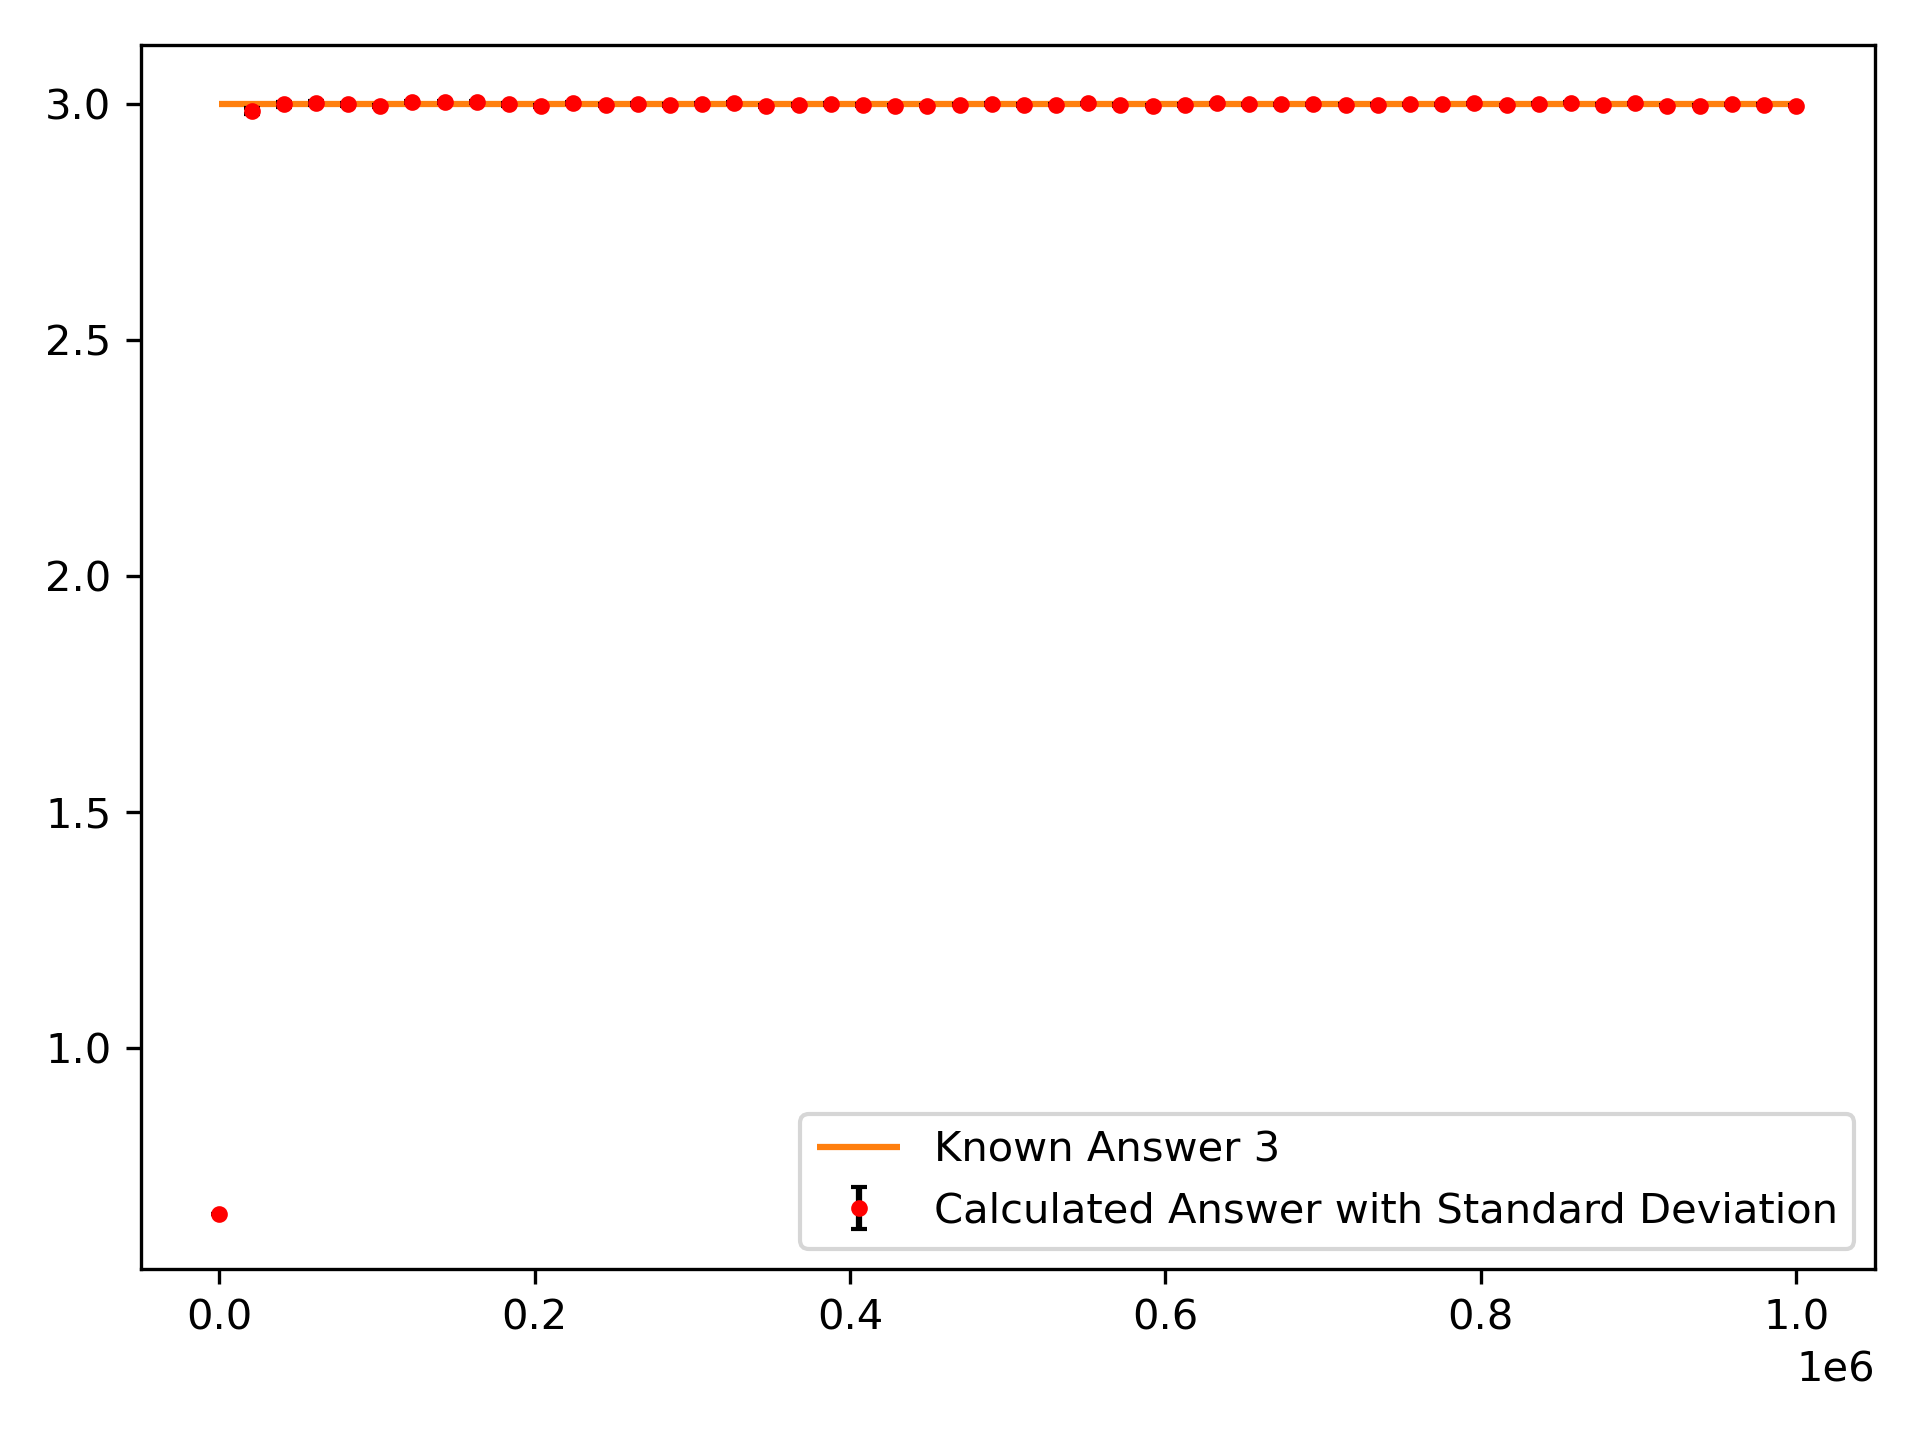
\includegraphics[width=0.7\textwidth]{task_6_b.png}
  \end{center}
  \caption{Plot showing the convergence of calculated guesses over a range of N random points (from $1$ to $10^6$)}
  \label{fig:task_6_b}
\end{figure}

\begin{figure}[H]
  \begin{center}
    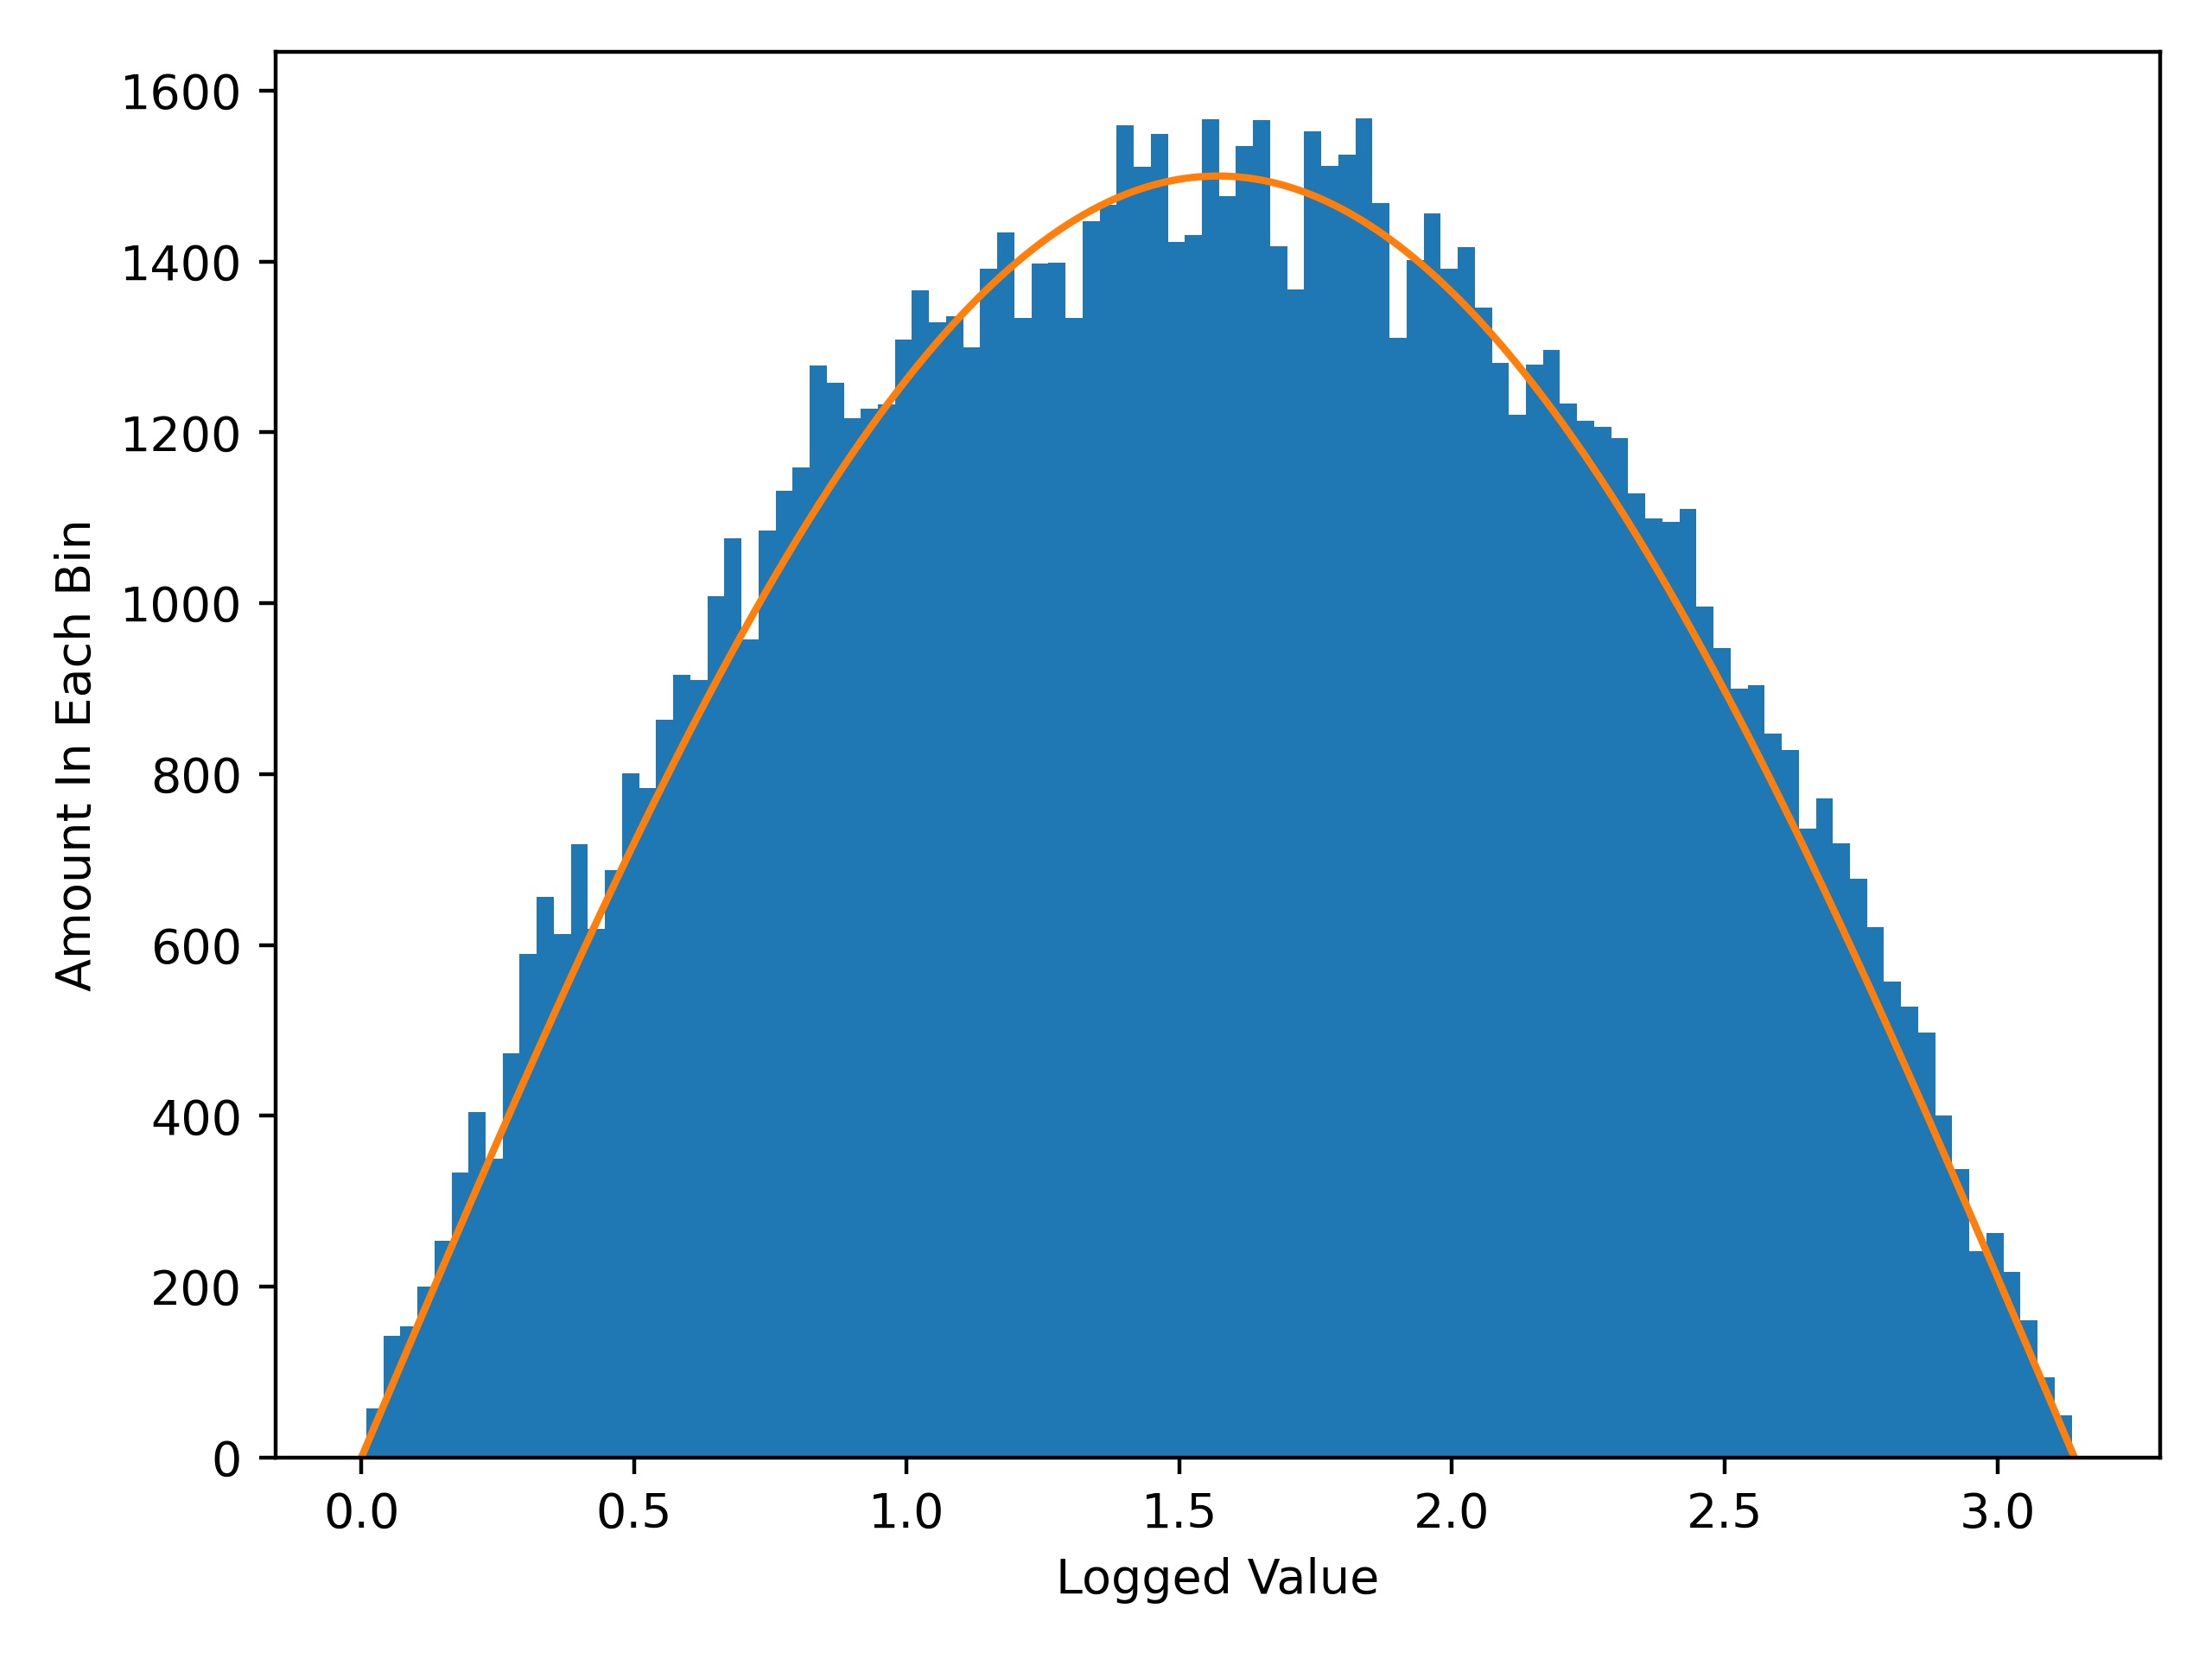
\includegraphics[width=0.7\textwidth]{histogram.jpg}
  \end{center}
  \caption{Histogram of Samples in Part b.}
  \label{fig:}
\end{figure}


\begin{figure}[H]
  \begin{center}
    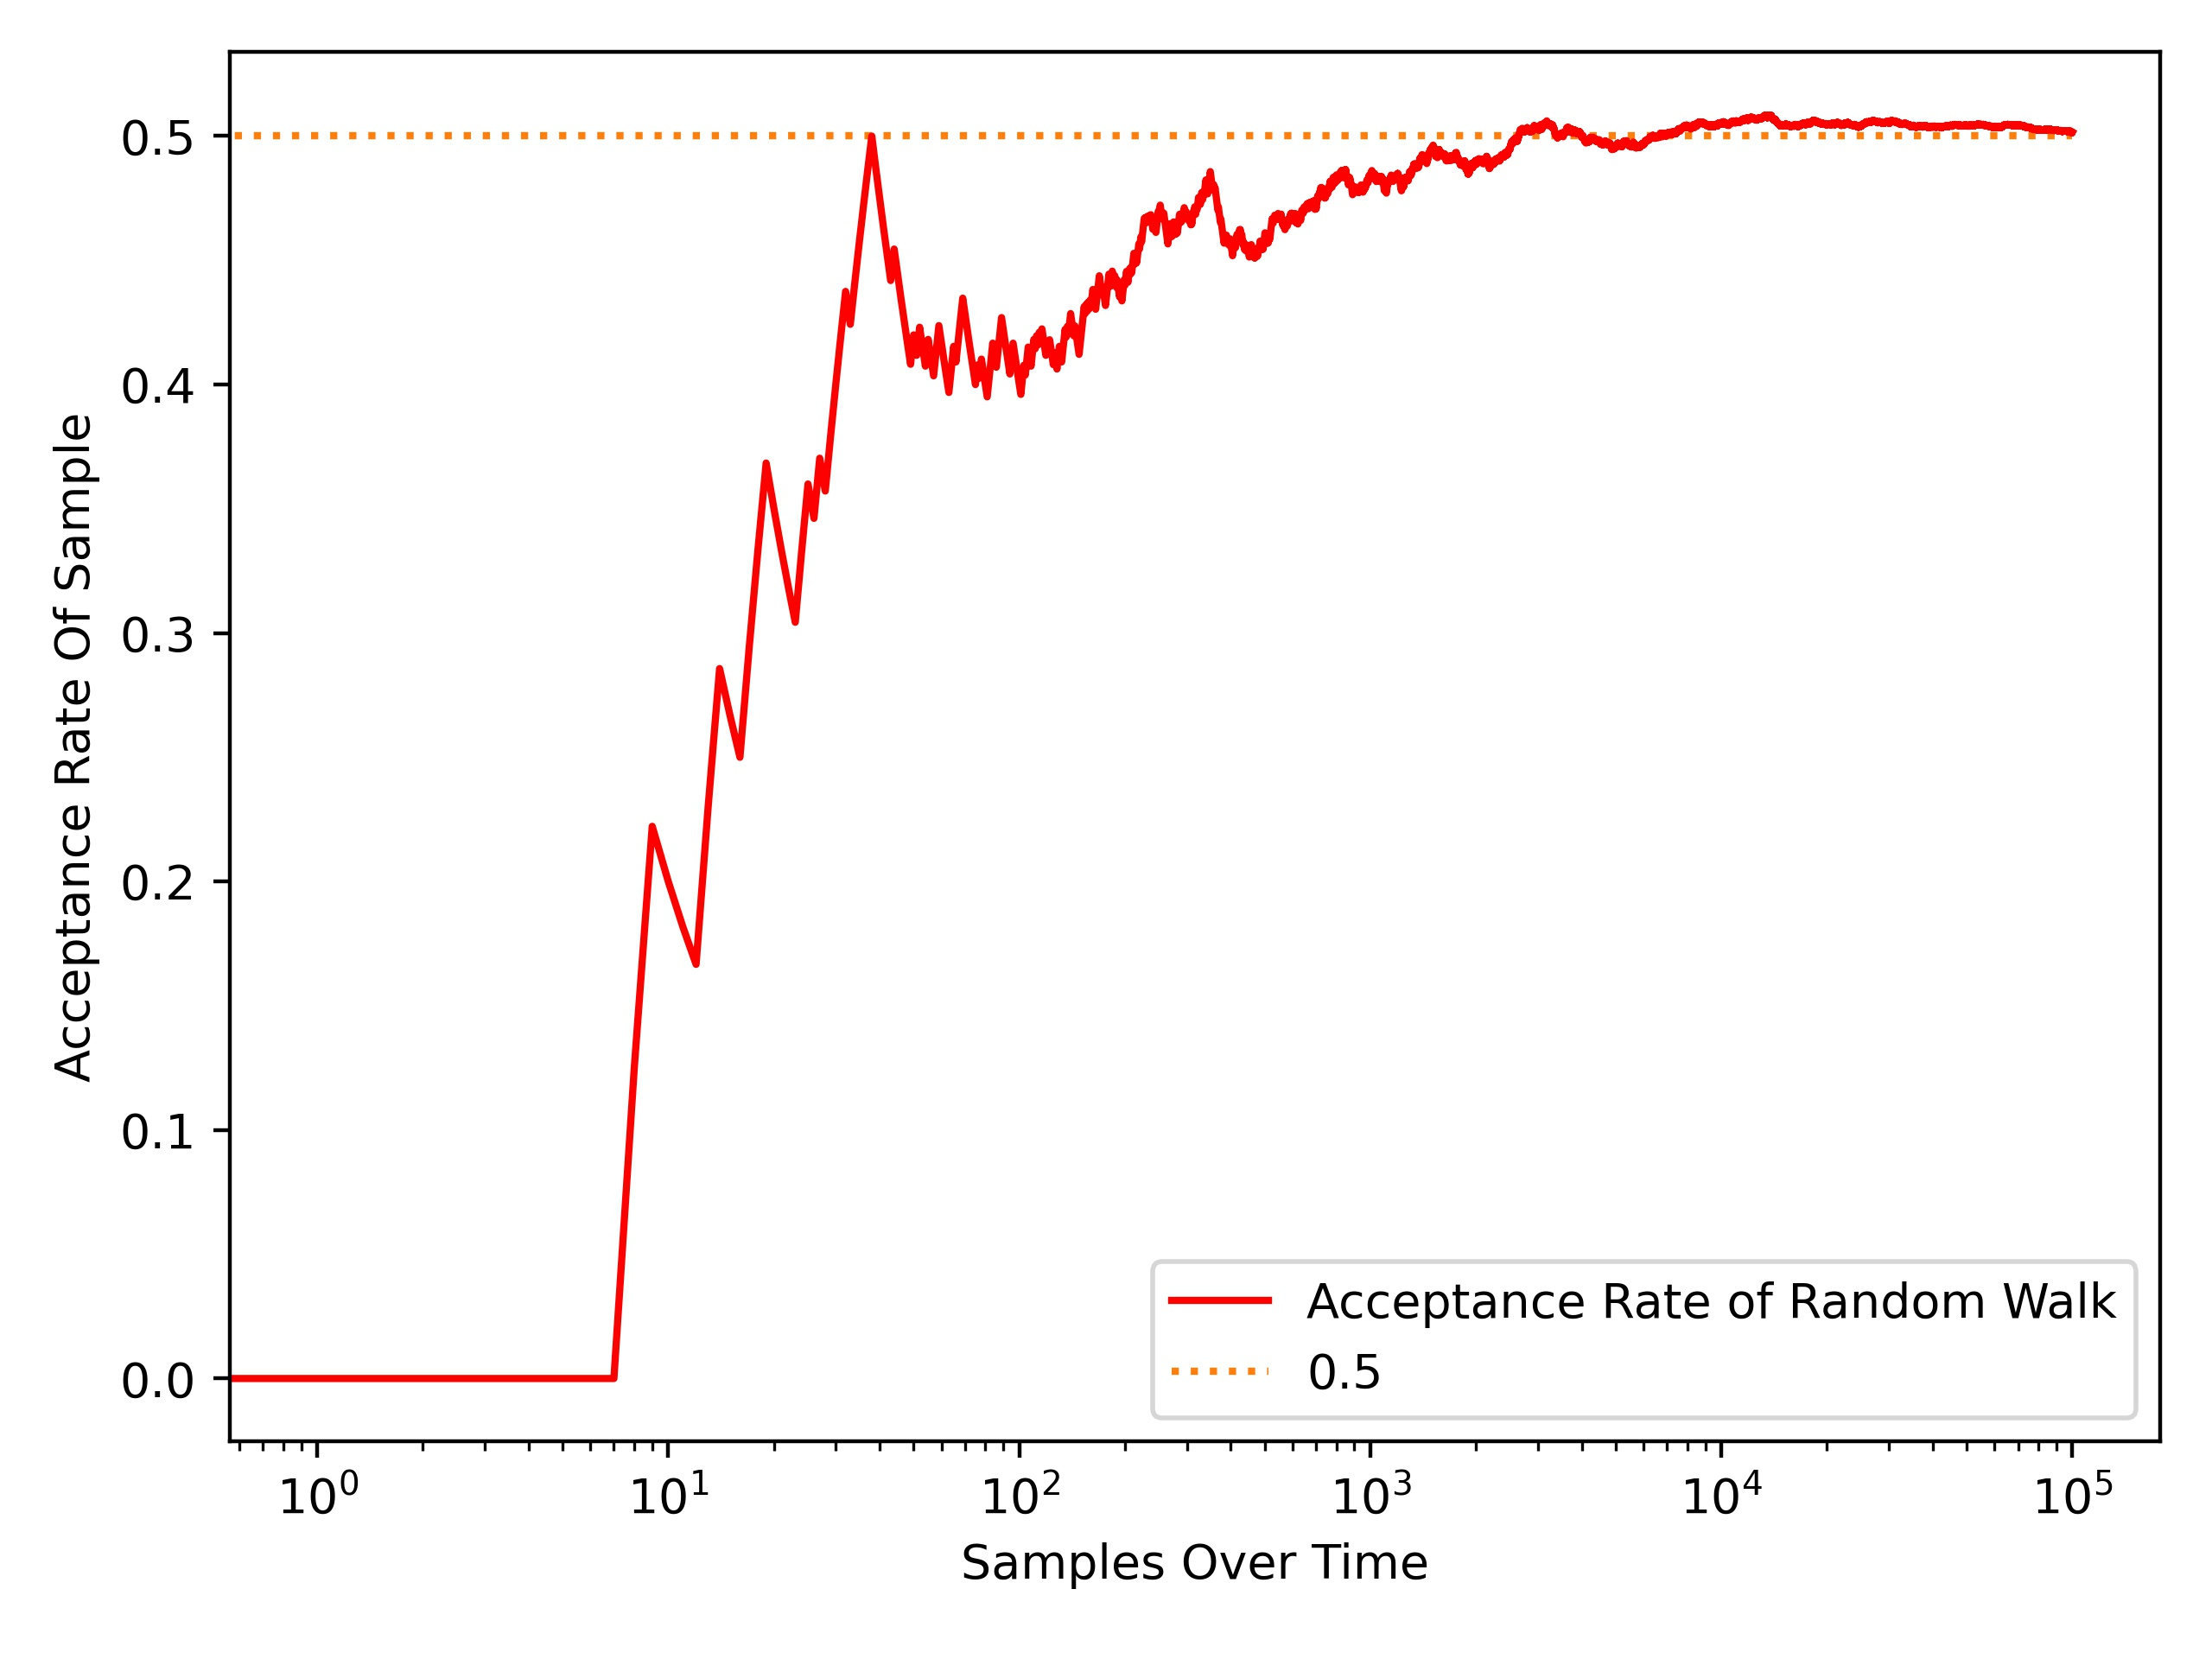
\includegraphics[width=0.7\textwidth]{Acceptance_Rate.jpg}
  \end{center}
  \caption{Figure showing the acceptance rate of the Metropolis method.}
  \label{fig:Acceptance_Rate}
\end{figure}



\end{document}
